\documentclass[
	% -- opções da classe memoir --
	12pt,				% tamanho da fonte
	openright,			% capítulos começam em pág ímpar (insere página vazia caso preciso)
	oneside,			% para impressão em verso e anverso. Oposto a oneside
	a4paper,			% tamanho do papel. 
	% -- opções da classe abntex2 --
	%chapter=TITLE,		% títulos de capítulos convertidos em letras maiúsculas
	%section=TITLE,		% títulos de seções convertidos em letras maiúsculas
	%subsection=TITLE,	% títulos de subseções convertidos em letras maiúsculas
	%subsubsection=TITLE,% títulos de subsubseções convertidos em letras maiúsculas
	% -- opções do pacote babel --
	english,			% idioma adicional para hifenização
	french,				% idioma adicional para hifenização
	spanish,			% idioma adicional para hifenização
	brazil				% o último idioma é o principal do documento
	]{abntex2}


% --- 
% CONFIGURAÇÕES DE PACOTES
% --- 
% ---
% Pacotes básicos 
% ---
\usepackage{lmodern}			% Usa a fonte Latin Modern			
\usepackage[T1]{fontenc}		% Selecao de codigos de fonte.
\usepackage[utf8]{inputenc}		% Codificacao do documento (conversão automática dos acentos)
\usepackage{lastpage}			% Usado pela Ficha catalográfica
\usepackage{indentfirst}		% Indenta o primeiro parágrafo de cada seção.
\usepackage{color}				% Controle das cores
\usepackage{graphicx}			% Inclusão de gráficos
\usepackage{microtype} 			% para melhorias de justificação
\usepackage{ufc-abntex2}
% ---
		
% ---
% Pacotes adicionais, usados apenas no âmbito do Modelo Canônico do abnteX2
% ---
\usepackage{lipsum}				% para geração de dummy text
% ---

% ---
% Pacotes de citações
% ---
\usepackage[brazilian,hyperpageref]{backref}	 % Paginas com as citações na bibl
\usepackage[alf]{abntex2cite}	% Citações padrão ABNT

% ---
% Configurações do pacote backref
% Usado sem a opção hyperpageref de backref
\renewcommand{\backrefpagesname}{Citado na(s) página(s):~}
% Texto padrão antes do número das páginas
\renewcommand{\backref}{}
% Define os textos da citação
\renewcommand*{\backrefalt}[4]{
	\ifcase #1 %
		Nenhuma citação no texto.%
	\or
		Citado na página #2.%
	\else
		Citado #1 vezes nas páginas #2.%
	\fi}%
% ---

% ---
% Configurações de aparência do PDF final

% alterando o aspecto da cor azul
\definecolor{blue}{RGB}{41,5,195}

% informações do PDF
\makeatletter
\hypersetup{
     	%pagebackref=true,
		pdftitle={\@title}, 
		pdfauthor={\@author},
    	pdfsubject={\imprimirpreambulo},
	    pdfcreator={LaTeX with abnTeX2},
		pdfkeywords={abnt}{latex}{abntex}{abntex2}{trabalho acadêmico}, 
		colorlinks=true,       		% false: boxed links; true: colored links
    	linkcolor=black,          	% color of internal links
    	citecolor=black,        		% color of links to bibliography
    	filecolor=magenta,      		% color of file links
		urlcolor=blue,
		bookmarksdepth=4
}
\makeatother
% --- 

% --- 
% Espaçamentos entre linhas e parágrafos 
% --- 

% O tamanho do parágrafo é dado por:
\setlength{\parindent}{1.3cm}

% Controle do espaçamento entre um parágrafo e outro:
\setlength{\parskip}{0.2cm}  % tente também \onelineskip

% ---
% compila o indice
% ---
\makeindex
% ---

\setlrmarginsandblock{3cm}{2cm}{*}
\setulmarginsandblock{3cm}{2cm}{*}
\checkandfixthelayout

\usepackage{float}
%\usepackage[a4paper,bottom=2cm,top=3cm,left=3cm,right=2cm]{geometry}


% Informações de dados para CAPA e FOLHA DE ROSTO
\titulo{\uppercase{Implantação de uma ferramenta de integração contínua em um Núcleo de Práticas em informática: Relato de Experiênca}}
\autor{Guylherme Tabosa Cabral}
\local{Quixadá, Ceará}
\data{2014}
\orientador{Prof Msc. Carlos Diego Andrade de Almeida}

% TODO: Fazer para SI, CC, ES
\instituicao{%
Universidade Federal do Ceará
\par
Campus Quixadá
\par
Curso de Engenharia de Software
}
\tipotrabalho{Trabalho de Conclusão de Curso (Monografia)}
\preambulo{Trabalho de Conclusão de Curso submetido à Coordenação do Curso de Engenharia de Software do Campus Quixadá da Universidade Federal do Ceará, como requisito parcial para obtenção do Título de Bacharel em Engenharia de Software.}


\begin{document}
\frenchspacing 

% ----------------------------------------------------------
% ELEMENTOS PRÉ-TEXTUAIS
% ----------------------------------------------------------
\pretextual
% Capa
\imprimircapa
% Folha de rosto (* indica que haverá a ficha bibliográfica)
%\imprimirfolhaderosto*

% Ficha Bibliográfica
%% ---
% Inserir a ficha bibliografica
% ---

% Isto é um exemplo de Ficha Catalográfica, ou ``Dados internacionais de
% catalogação-na-publicação''. Você pode utilizar este modelo como referência. 
% Porém, provavelmente a biblioteca da sua universidade lhe fornecerá um PDF
% com a ficha catalográfica definitiva após a defesa do trabalho. Quando estiver
% com o documento, salve-o como PDF no diretório do seu projeto e substitua todo
% o conteúdo de implementação deste arquivo pelo comando abaixo:
%
% \begin{fichacatalografica}
%     \includepdf{fig_ficha_catalografica.pdf}
% \end{fichacatalografica}
\begin{fichacatalografica}
	\vspace*{\fill}					% Posição vertical
	\hrule							% Linha horizontal
	\begin{center}					% Minipage Centralizado
	\begin{minipage}[c]{12.5cm}		% Largura
	
%	\imprimirautor
	Cabral,Guylherme Tabosa
	
	\hspace{0.5cm} \imprimirtitulo  / \imprimirautor. --
	\imprimirlocal, \imprimirdata-
	
	\hspace{0.5cm} \pageref{LastPage} p. : il. (algumas color.) ; 30 cm.\\
	
	\hspace{0.5cm} \imprimirorientadorRotulo~\imprimirorientador\\
	
	\hspace{0.5cm}
	\parbox[t]{\textwidth}{\imprimirtipotrabalho~--~\imprimirinstituicao,\imprimirlocal,
	\imprimirdata.}\\
	
	\hspace{0.5cm}
		1. Gerência de Configuração.
		2. Integração Contínua.
		3. Processo de Software.
		4. Qualidade de Software
		I. Almeida, Carlos Diego Andrade de.
		II. Universidade Federal do Ceará.
		III. \imprimirtitulo.\\ 			
	
	\hspace{8.75cm} CDU 02:141:005.7\\
	
	\end{minipage}
	\end{center}
	\hrule
\end{fichacatalografica}
% ---

% Errata
%% ---
% Inserir errata
% ---
\begin{errata}
Elemento opcional da NORMA. Exemplo:

\vspace{\onelineskip}

FERRIGNO, C. R. A. \textbf{Tratamento de neoplasias ósseas apendiculares com
reimplantação de enxerto ósseo autólogo autoclavado associado ao plasma
rico em plaquetas}: estudo crítico na cirurgia de preservação de membro em
cães. 2011. 128 f. Tese (Livre-Docência) - Faculdade de Medicina Veterinária e
Zootecnia, Universidade de São Paulo, São Paulo, 2011.

\begin{table}[htb]
\center
\footnotesize
\begin{tabular}{|p{1.4cm}|p{1cm}|p{3cm}|p{3cm}|}
  \hline
   \textbf{Folha} & \textbf{Linha}  & \textbf{Onde se lê}  & \textbf{Leia-se}  \\
    \hline
    1 & 10 & auto-conclavo & autoconclavo\\
   \hline
\end{tabular}
\end{table}

\end{errata}
% ---


% Folha de Aprovação
%% ---
% Inserir folha de aprovação
% ---

% Isto é um exemplo de Folha de aprovação, elemento obrigatório da NBR
% 14724/2011 (seção 4.2.1.3). Você pode utilizar este modelo até a aprovação
% do trabalho. Após isso, substitua todo o conteúdo deste arquivo por uma
% imagem da página assinada pela banca com o comando abaixo:
%
% \includepdf{folhadeaprovacao_final.pdf}
%
\begin{folhadeaprovacao}

  \begin{center}
    {\ABNTEXchapterfont\bfseries\Large\imprimirautor}
    \vspace{1cm}

    \begin{center}
      \ABNTEXchapterfont\bfseries\Large\imprimirtitulo
    \end{center}

    \vspace{2cm}
    \begin{minipage}{\textwidth}
        \imprimirpreambulo
        \\ \\ \\
        Aprovada em: \_\_/\_\_/\_\_\_\_
    \end{minipage}%
     
    \vspace{2cm}
	\textbf{BANCA EXAMINADORA}
   \end{center}
	

   \assinatura{\imprimirorientador \space (Orientador) \\ Universidade Federal do Ceará (UFC)}
   \assinatura{\imprimircoorientador \space (Membro) \\ Universidade Federal do Ceará (UFC)}
   \assinatura{Professor Msc. Da Silva \\ Universidade Federal do Ceará (UFC)}
   %\assinatura{\textbf{Professor} \\ Convidado 2}
   %\assinatura{\textbf{Professor} \\ Convidado 3}
      
%   \begin{center}
%    \vspace*{0.5cm}
%    {\large\imprimirlocal}
%    \par
%    {\large\imprimirdata}
%    \vspace*{1cm}
%  \end{center}
  
\end{folhadeaprovacao}
% ---

%\imprimirfolhadeaprovacao

% Dedicatória
%% ---
% Dedicatória
% ---
\begin{dedicatoria}
   \vspace*{\fill}
   	\begin{flushright}
   \noindent
    Dedico este trabalho a minha família principalmente meus avós, minha mãe, meu irmão e meu pai.
   	\end{flushright}
\end{dedicatoria}
% ---

% Agradecimentos
%% ---
% Agradecimentos
% ---
\begin{agradecimentos}
	 Agradeço primeiramente a Deus por me dar sabedoria e vontade para concluir este trabalho.A minha mãe Rejane, pelo exemplo de mulher e por sempre olhar por mim quando não estive perto durante esses anos de universidade. A meus avós Rita e Nonato por todo o apoio, amor e por serem meu maior exemplo de vida. A meu irmão Felype por sempre partilhar comigo momentos bons e ruins e cuidar de mim quando precisei. A meu pai João por ensinar que o trabalho sempre gera resultados, que o esforço é seu maior aliado para o sucesso. A minha família pela ajuda e cuidado. A minha namorada Mikaely por ter me aturado nos momentos de confusão, medo, raiva angústia e outros mais, sua presença ao meu lado me fez mais forte e focado nos objetivos. A meus amigos de faculdade, por todos esses anos de companheirismo, felicidades ajudas. A meu orientador Carlos Diego por me guiar na obtenção do melhor resultado possível e disponibilidade e interesse neste projeto. A UFC e seus funcionários por fornecer as ferramentas para que pudesse evoluir meus conhecimentos. Obrigado a todos.
\end{agradecimentos}
% ---

% Epígrafe
%% ---
% Epígrafe
% ---
\begin{epigrafe}
    \vspace*{\fill}
	\begin{flushright}
		\textit{``Observo a mim mesmo em silêncio, \\
		porque é nele onde mais e melhor se diz, \\
		Me  ensino a ser mais tolerante, não julgar ninguém \\
		E com isso ser mais feliz.\\
		''}
	\end{flushright}
\end{epigrafe}
% ---

% RESUMOS
%% resumo em português
\setlength{\absparsep}{18pt} % ajusta o espaçamento dos parágrafos do resumo
\begin{resumo}
 Segundo a NBR6028:2003, o resumo deve ressaltar o
 objetivo, o método, os resultados e as conclusões do documento. A ordem e a extensão
 destes itens dependem do tipo de resumo (informativo ou indicativo) e do
 tratamento que cada item recebe no documento original. O resumo deve ser
 precedido da referência do documento, com exceção do resumo inserido no
 próprio documento. (\ldots) As palavras-chave devem figurar logo abaixo do
 resumo, antecedidas da expressão Palavras-chave:, separadas entre si por
 ponto e finalizadas também por ponto.

 \textbf{Palavras-chaves}: Integração Contínua. Desenvolvimento Ágil. Gerenciamento de Configuração.
\end{resumo}
%% resumo em inglês
\begin{resumo}[Abstract]
 \begin{otherlanguage*}{english}
The agile development is day by day inserted on the quotidian of software development companies. The growing seek for agility in the development and market competitiveness has impacted in the existence of this scenario. Therefore, many companies seek to apply the defined methodologies in this kind of development	in their processes, however, this is not an easy task. The definition and deployment of this practices executed in a way not adequate enough can bring contrary results to the expected. So, this work had as an aim to implant the using of a continuous integration tool on a software factory, the Informatics Practice Center (NPI) at UFC in Quixadá. A continuous integration tool is inserted in one of the practices defined by Extreme Programming (XP). In order to reach this goals, the current process of NPI was analyzed, beyond the author experience thas was a member of this software factory. Added to this stage was defined the continuous integration tool to be implanted according with a set of specified characteristics, the knowledges of the factory's members about Configuration Management and Continuous Integration was evaluated, and finally the deployment, with the definition of positives and negatives points found at the deployment.

   \vspace{\onelineskip}
 
   \noindent 
   \textbf{Key-words}: Continuous Integration. Agile Development. Configuration Management.
 \end{otherlanguage*}
\end{resumo}
%% resumo em francês 
\begin{resumo}[Résumé]
 \begin{otherlanguage*}{french}
    Il s'agit d'un résumé en français.
 
   \textbf{Mots-clés}: latex. abntex. publication de textes.
 \end{otherlanguage*}
\end{resumo}

%% resumo em espanhol
\begin{resumo}[Resumen]
 \begin{otherlanguage*}{spanish}
   Este es el resumen en español.
  
   \textbf{Palabras clave}: latex. abntex. publicación de textos.
 \end{otherlanguage*}
\end{resumo}
% ---

% Lista de ilustrações
\pdfbookmark[0]{\listfigurename}{lof}
\listoffigures*
\cleardoublepage

% Lista de tabelas
\pdfbookmark[0]{\listtablename}{lot}
\listoftables*
\cleardoublepage

% Abreviaturas e Siglas
%% Lista de abreviaturas e siglas
% ---
\begin{siglas}
  \item[NPI] Núcleo de Práticas em Informática
  \item[CMMI] Capability Maturity Model Integration
  \item[MPS.BR] Melhoria de Processo Brasileiro
  \item[GC] Gerência de Configuração
  \item[SCV] Sistema de Controle de Versão
  \item[SCM] Sistema de Controle de Mudança
  \item[IC]  Integração Contínua
  \item[UFC] Universidade Federal do Ceará
  \item[TI] Tecnologia da Informação
  \item[SGBD] Sistemas de Gerência de Banco de Dados
  \item[CCB] Change Control Board
  \item[SBC] Sociedade Brasileira de Computação
\end{siglas}
% ---

% Símbolos
%%Lista de símbolos
% ---
\begin{simbolos}
  \item[$ \Gamma $] Letra grega Gama
  \item[$ \Lambda $] Lambda
  \item[$ \zeta $] Letra grega minúscula zeta
  \item[$ \in $] Pertence
\end{simbolos}
% ---

% Sumário
\pdfbookmark[0]{\contentsname}{toc}
\tableofcontents*
\cleardoublepage

% ----------------------------------------------------------
% ELEMENTOS TEXTUAIS
% ----------------------------------------------------------
\textual

% ----------------------------------------------------------
% Introdução (exemplo de capítulo sem numeração, mas presente no Sumário)
% ----------------------------------------------------------
\chapter{Introdução}
% ----------------------------------------------------------

O presente trabalho visa implantar no Núcleo de Práticas em Informática da Universidade Federal do Ceará do Campus de Quixadá (NPI) a utilização de uma ferramenta de Integração Contínua (IC), buscando analisar as taxas de manutenibilidade dos sistemas de software produzidos e avaliar o impacto que esta ferramenta possui sobre a manutenibilidade de um sistema de software.

O NPI é o local onde estudantes que estão em ano de conclusão de curso podem estagiar e aprimorar seus conhecimentos adquiridos no decorrer do curso além de concluir seus componentes curriculares obrigatórios. Este surgiu devido à pouca demanda de empresas de Tecnologia da Informação (TI) na região onde a universidade se encontra, em Quixadá no Ceará. Dentro do NPI, os projetos desenvolvidos têm como objetivo construir soluções que facilitem as atividades do cotidiano da universidade, esta que tem um grande interesse no desenvolvimento destes projetos, pois consegue reduzir custos ao priorizar construções de sistemas internamente \cite{npi2013}. Em paralelo, aumenta a qualidade dos profissionais formados por ela, além de proporcionar um ambiente real de trabalho que facilita a entrada dos concludentes no mercado de trabalho.

Dentro do NPI existe um modelo de processo definido em que os desenvolvedores devem seguir para o exercício de suas atividades \cite{npi2013}. Entretanto, este não é devidamente seguido, ocasionando uma despadronização na maneira como estes  desenvolvedores trabalham em seus projetos. Somado-se a isto, o NPI apresenta problemas tais como: "Baixa qualidade da documentação dos sistemas; [\ldots] Falta de uma equipe de manutenção; [\ldots] Rotatividade dos profissionais" o que acaba gerando graves problemas de manutenção \cite[p.~4]{paduelli2006}.


Segundo \citeonline[p.~170]{sommerville2011}, "a manutenção de software é o processo geral de mudança em um sistema depois que ele é liberado para uso". Sendo assim, entende-se como manutenção de software  qualquer alteração realizada no sistema após este ser considerado "pronto" e implantado em seu ambiente de operação. Atualmente, esta vem ganhando uma maior atenção por parte das empresas desenvolvedoras de software. Isso acontece devido aos altos custos na fase de manutenção, podendo atingir 70\% do esforço total aplicado no projeto, além de sofrer possíveis aumentos ao longo da produção do software \cite{pressman2010}.

Mudanças no software são inevitáveis, e não possuem regra, simplesmente acontecem. Garantir que essas mudanças sejam devidamente controladas, identificadas é o papel da  Gerência de Configuração (GC), esta que tem sua importância evidenciada quando diferentes modelos de maturidade o abordam como MPS.BR no nível F e o CMMI(Capability Maturity Model Integration) \cite{furlaneto2006}. Para identificar e auxiliar no controle das mudanças, um conjunto de ferramentas CASE (Computer-Aided Software Engineering) são utilizadas pela Gerência de Configuração.

A experiência em aplicar ferramentas  de gestão de configuração com o objetivo de melhorar a manutenibilidade de uma fábrica de software é explanado por \citeonline{poliana2005}. Eles inseriram a utilização destas ferramentas para evitar a inserção de novos erros proveniente de manutenções realizadas no software. Diferentemente do trabalho a ser desenvolvido nesse projeto que busca verificar o impacto de uma ferramenta em específico, de Integração Contínua,  na melhoria da manutenibilidade.

Entende-se Integração Contínua como uma ferramenta de gestão de configuração, que auxilia os desenvolvedores e permite que as mudanças realizadas no software sejam imediatamente avaliadas, testadas, verificadas de modo a prover um  \textit{feedback} imediato para correção de possíveis erros de integração que somente seriam verificados futuramente após problemas mais complexos de integração \cite{paul2007}.

A justificativa pela escolha do tema se deu através da ausência de pesquisas que busquem avaliar o impacto que o uso de uma ferramenta de integração contínua utilizada durante desenvolvimento de um produto de software exerce sobre a manutenibilidade do software produzido. As buscas por pesquisas foram realizadas no: acervo da Sociedade Brasileira de Computação (SBC), \textit{Google Academys} utilizando os termos: \textit{Continuous Integration, Continuous Integration and maintainability index}. Proporcionar conhecimento para o mercado de modo a ajudar empresas a avaliarem a necessidade, viabilidade do uso de ferramentas deste gênero.

% ----------------------------------------------------------
% PARTE I
% ----------------------------------------------------------
%\part{Preparação da pesquisa}

% Capitulo com exemplos de comandos inseridos de arquivo externo 
\chapter{Fundamentação Teórica}\label{fundamentacao}
Nesta seção será apresentado os conceitos necessários para um completo entendimento deste trabalho. A \autoref{gerenciadeconfiguracao} conceitos inerentes a Gerência de configuração, juntamente com algumas ferramentas CASE e com ênfase em Integração Contínua descrito na \autoref{integracaocont} e por fim na \autoref{processonpi} será descrito o processo de gerência de configuração do NPI.

\section{Gerência de Configuração}\label{gerenciadeconfiguracao}
A gerência de configuração é a área da engenharia de software responsável pela evolução do software. Ela atua durante todo o ciclo de vida do produto de software e, por meio de técnicas, ferramentas e metodologias, visa garantir que as mudanças que irão ocorrer dentro do ciclo de vida do desenvolvimento do software sejam identificadas, avaliadas e comunicada a todos os envolvidos através de ferramentas que auxiliam neste processo de evolução.
Portanto "o propósito do processo de Gerência de Configuração é estabelecer e manter a integridade de todos os produtos de trabalho de um processo ou projeto e disponibilizá-la a todos os envolvidos"\space\cite{mpsbr}.
\subsection{Plano de Gerenciamento de Configuração}\label{pgc}
O Plano de Gerenciamento de Configuração (PGC) descreve todas as atividades de configuração e mudança que serão realizadas durante o projeto. Um conjunto de atividades, responsabilidades, ferramentas, recursos e etc. A gerência de configuração tem como objetivo garantir a integridade dos itens de configuração, que são qualquer artefato que esteja sob custódia da Gerência de Configuração, através do versionamento, da identificação, controlando mudanças e acesso. 

\subsection{Sistema de Controle de Versão}
Um sistema de controle de versão: "	[...] combina procedimentos e ferramentas para gerenciar diferentes versões de objetos de configurações que são criadas durante o processo de engenharia de software" \cite[p.~927]{pressman2010}.
Atualmente, o uso de sistema de controle de versão se tornou comum nas empresas de grande e pequeno porte. Tais ferramentas permitem que se tenha o controle de diferentes versões de arquivos que estão submetidos ao versionamento, recuperação de versões antigas, visualizar alterações realizadas em arquivos e saber por quem e quando o arquivo foi alterado. Através de comandos (i.e.,\textit{check-in},\textit{check-out}) os usuários conseguem se comunicar com o repositório a fim de obter os artefatos ali armazenados \cite{gleiph2011}. Em situações especais faz-se necessário que os desenvolvedores trabalhem em una linha diferente da original chamada de \textit{mainline}, geralmente essa situação ocorre quando tem-se como objetivo consertar bugs de versões anteriores do repositório, nesse caso um \textit{branch}, uma ramificação na linha de desenvolvimento do controle de versão, é criado afim de permitir a realização desta ação, permitindo assim o trabalho em paralelo sobre o mesmo repositório.
\begin{figure}[h]
\centering
\caption[Branch no Sistema de Controle de Versão]{Branch no Sistema de Controle de Versão.}
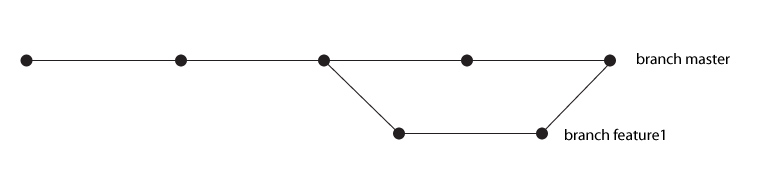
\includegraphics[width=0.5\linewidth]{./images/branch}
\label{fig:Branch}
\legend {\fontsize{10}{12}\selectfont {Fonte: \citeonline{tableless2012}}.}
\end{figure}
A figura \autoref{fig:Branch} demonstra a criação de um \textit{branch} paralelo a linha de desenvolvimento principal chamada de branch feature1 e branch master respectivamente, posteriormente as ações realizadas no \textit{branch feature1} são incorporadas ao \textit{branch master}.
\subsubsection{Sistema de Controle de Versão Local}
Um sistema de controle de versão local	armazenam todas as informações de um arquivo submetido ao versionamento na máquina local, guardando diferentes versões daquele arquivo localmente como demonstrado na figura \autoref{fig:SCVLocal}.
\begin{figure}[h]
\centering
\caption[Sistema de Controle de Versão Local]{Sistema de Controle de Versão Local.}
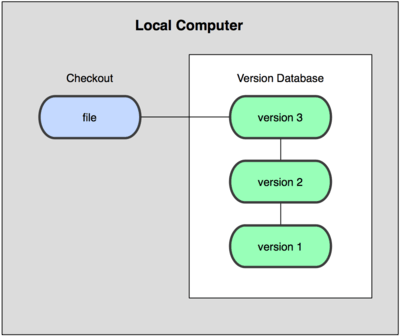
\includegraphics[width=0.5\linewidth]{./images/scvlocal}
\label{fig:SCVLocal}
\legend {\fontsize{10}{12}\selectfont {Fonte:\cite{git}}.}
\end{figure}
\subsubsection{Sistema de Controle de Versão Centralizado} Sistema de controle de versão centralizado como o nome diz possuem um único servidor centralizado, como o \textit{subversion} \footnote{http://subversion.apache.org}, \textit{perforce} \footnote{http://www.perforce.com}, este tipo de padrão de SCV mantém em seu único servidor todos os arquivos versionados. Para cada comando de comunicação realizado nos arquivos versionados, uma requisição deverá ser feita, podendo gerar lentidão ou deixar o servidor fora de funcionamento.
\begin{figure}[h]
\centering
\caption[Sistema de Controle de Versão Centralizado]{Sistema de Controle de Versão Centralizado.}
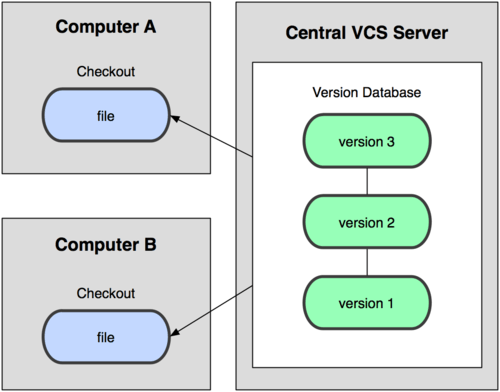
\includegraphics[width=0.5\linewidth]{./images/scvcentral}
\label{fig:SCVCentral}
\legend {\fontsize{10}{12}\selectfont {Fonte: \citeonline{git}}.}
\end{figure}
No exemplo acima dois desenvolvedores trabalhando em máquinas diferentes realizam a comunicação com o servidor central para obter o artefato de trabalho.	
\subsubsection{Sistema de Controle de Versão Distribuído}Os sistemas de controle de versão distribuído possuem um servidor central onde os arquivos são submetidos a versionamento, entretanto cada desenvolvedor possui em sua máquina de trabalho as versões que estavam no servidor, tornando cada \textit{workstation} um "servidor", portanto, caso ocorra um problema no servidor central, estes podem ser recuperados via \textit{workstation}, mantendo a integridade dos arquivos e evitando ser um ponto único de falha, como mostra a figura \autoref{fig:SCVDistribuido}.
\begin{figure}[H]
\centering
\caption[Sistema de Controle de Versão Distribuído]{Sistema de Controle de Versão Distribuído.}
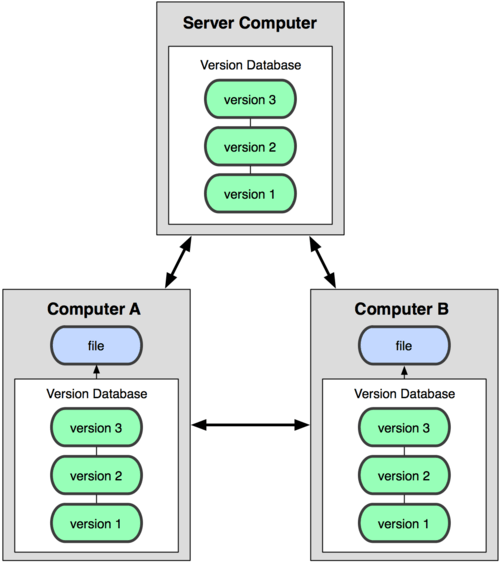
\includegraphics[width=0.5\linewidth]{./images/scvdist}
\label{fig:SCVDistribuido}
\legend {\fontsize{10}{12}\selectfont {Fonte: \citeonline{git}}.}
\end{figure}
\space

\subsection{Sistema de Controle de Mudança}
Todo software sofre mudanças, lidar com as mudanças é o papel da gerência de configuração, e para isso o gerente de configuração utiliza de um sistemas de controle de mudança. "O controle de mudança combina procedimentos humanos e ferramentas automatizadas para proporcionar um mecanismo de controle de mudança"\space \citeonline[p~.930]{pressman2010}. As mudanças devem ser avaliadas com cautela baseando-se, em seu custo benefício, uma combinação de esforço e \textit{business value}. A mudança tem início quando um "cliente" solicita a mudanças através de um formulário, conhecido como \textit{change request}. Nesse formulário é descrito os aspectos da mudança, após a solicitação ser realizada, esta deve ser avaliada, verificando se a mesma já foi solicitada, ou corrigida em caso de \textit{bugs}. Após a mudança ser validada, uma equipe de desenvolvedores avaliam os impactos que esta mudança têm sobre o sistema, verificando custo/benefício e esforço de realização \cite{sommerville2011}. Posterior a essa análise, a mudança será avaliada por um comitê de controle de mudança (CCB) que avaliará o impacto da perspectiva do negócio, o que decidirá se esta mudança será revisada, aprovada ou reprovada. Alguns sistemas que fornecem este controle sobre as mudança são: \textit{redmine \footnote{http://www.redmine.org}, GitHub \footnote{http://www.github.com} Jira \footnote{https://www.atlassian.com/software/jira}}
\subsection{Auditoria de Configuração}
"Uma auditoria de configuração de software complementa a revisão técnica formal ao avaliar um objeto de configuração quanto às características que geralmente não são consideradas durante a revisão"\space\citeonline[p~.934]{pressman2010}. Ela tem como objetivo garantir que mesmo com as mudanças realizadas a qualidade foi mantida. As auditorias se dividem em dois tipos: auditorias funcionais e auditorias físicas, a auditoria física baseia-se em verificar se os itens de configuração estão devidamente atualizados e se as práticas e padrões foram realizados da maneira correta, enquanto a auditoria funcional, busca verificar os aspectos lógicos dos itens de configuração.
\subsection{Ferramentas de Build}
As ferramentas de build tem como objetivo automatizar processos repetitivos, aumentando a produtividade e facilitando o trabalho do desenvolvedor. Através da definição de uma rotina, ou conjunto de comandos, o desenvolvedor informa a ferramenta que tipo de processo ele deseja automatizar, pode ser desde compilar e testar uma classe, como dropar e criar uma tabela nova no banco de dados, comprimir arquivos css e javascript, cabe ao desenvolvedor definir o escopo da automatização. Alguns exemplo deste tipo de ferramenta são: \textit{Ant, Grunt, Gulp, Maven}.


\begin{figure}[H]
\centering
\caption[Processo Lógico de uma Build]{Processo Lógico de uma Build.}
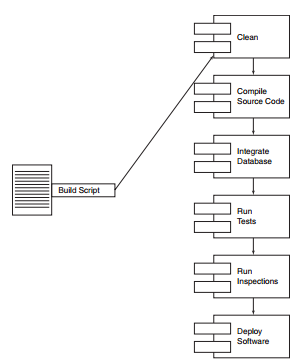
\includegraphics[scale=0.9]{./images/build}
\label{fig:build}
\legend {\fontsize{10}{12}\selectfont {Fonte: \citeonline{paul2007}}.}
\end{figure}
Na figura \autoref{fig:build} um script foi definido para realizar as seguintes funções, será realizado um clean no projeto, compilará o código fonte, integrará com o banco de dados, executará testes e inspeções no código e por fim será realizado o \textit{deploy} da aplicação.


%\subsection{Ferramentas de Integração Contínua}

\section{Integração Contínua}\label{integracaocont}
\begin{OnehalfSpace}
A integração contínua tem como objetivo identificar erros o mais rapidamente, permitindo que alterações efetuadas e integradas aos repositórios dos sistemas de controle de versão (SCV) sejam posteriormente verificadas e caso erros ocorram, estes sejam notificados imediatamente ao autor da alteração.
A melhor definição a cerca de integração contínua foi definida por \citeonline{fowler2000}
\end{OnehalfSpace}

\begin{citacao}
"[...] uma prática de desenvolvimento de software onde os membros de um time integram seu trabalho frequentemente, geralmente cada pessoa integra pelo menos diariamente – podendo haver múltiplas integrações por dia. Cada integração é verificada por uma build automatizada (incluindo testes) para detectar erros de integração o mais rápido possível. Muitos times acham que essa abordagem leva a uma significante redução nos problemas de integração e permite que um time desenvolva software coeso mais rapidamente." \citeonline[tradução nossa]{fowler2000}.
\end{citacao}

\subsection{Características de Integração}
Os requisitos para utilizar uma ferramenta de integração contínua de acordo com \citeonline{Anti2010} são:
\begin{itemize}
\item {\textbf{Uma conexão com um sistema de controle de versão:}}

A integração contínua necessita desta conexão, pois ela identifica as alterações ocorridas no repositório e dá início ao processo de integração.

\item {\textbf{A definição de uma build:}}

A integração contínua possui uma build privada que será executada assim que o processo de integração for iniciado, e é esta build que define que ações serão realizadas no processo de integração, tais como compilação, testes, análise de código.
\item {\textbf{Um mecanismo de feedback:}}

Um dos principais objetivos da integração contínua consiste em seu \textit{feedback} imediato, sendo assim um mecanismo deste tipo é essencial para a ferramenta, tais como e-mail, sms.
\item {\textbf{Um processo de integração do código: }}
O processo de integração consiste em como esta será realizada, manualmente ou através de um servidor de integração contínua de forma automatizada.

\end{itemize}

\subsection{Processo de Integração}
A integração ocorre quando alguma mudança é enviada ao sistema de controle de versão do repositório, que através de um servidor de integração contínua identifica a mudança e executa sua build privada \cite{mraz2013}. 


\begin{figure}[H]
\centering
\caption[Ambiente de Integração Contínua]{Ambiente de Integração Contínua.}
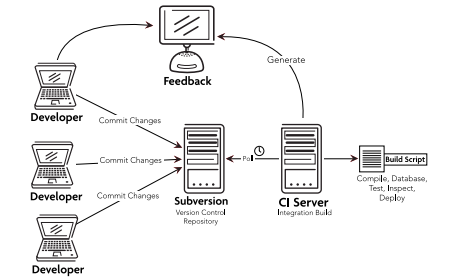
\includegraphics[scale=1.0]{./images/CI}
\label{fig:CI}
\legend {\fontsize{10}{12}\selectfont Fonte: \citeonline{paul2005}.}
\end{figure}

A \autoref{fig:CI} descreve um ambiente em que um servidor de integração contínua é utilizado. Existem três ambientes de trabalho distintos formado por três desenvolvedores que obtiveram uma cópia do projeto do repositório do SCV para trabalharem em suas \textit{workstation}, durante o trabalho alterações foram realizadas e commitadas ao repositório central, após a inserção junto ao repositório o servidor de integração contínua verifica as alterações e executa uma build de integração,  caso exista um problema com a build e esta não seja bem sucedida, o responsável pela alteração será informado sobre o ocorrido, assim seu objetivo em diante será a correção da build.

\subsection{Benefícios da Integração Contínua}

As principais vantagens em utilizar um servidor de integração contínua segundo \citeonline[p.~29]{paul2007} são:

\begin{itemize}
\item {\textbf{Redução de Riscos}}: 
Através da detecção imediada de código quebrados, ou incorretos, reduz-se risco atrelados ao produto.
\item {\textbf{Redução de processos manuais repetitivos}}:
Um conjunto de tarefas são executadas automaticamente pela build privada do servidor de integração contínua.
\item {\textbf{Permitir melhor visibilidade do projeto}}:
Através da identificação de informações inerentes ao desenvolvimento, como frequência de códigos defeituosos, módulos mais complexos, permitindo maior gerenciamento do projeto.
\item {\textbf{Estabelecer uma maior confiança no produto do time de desenvolvimento}}:
Através da visualizações de mudanças bem sucedidas, os desenvolvedores sentem maior confiança ao realizarem mudanças.
\end{itemize}

%\subsection{Integração Contínua e a Redução de Riscos}
%Os Riscos em produtos de software estão diretamente relacionados. Segundo \citeonline[p~.48]{paul2007} se você consegue reduzir certos riscos no software, você pode melhorar a qualidade do software.
\subsection{Builds Automatizadas}
Builds são rotinas de execução definidas com o objetivo de reduzir processos repetitivos. Durante o processo de desenvolvimento de um software muitas ações tendem a serem repetidas por parte dos desenvolvedores, utilizar o tempo para a realização  de atividades que poderiam ser automatizadas, de forma manual, reduz a produtividade e preocupações com melhorias devido ao tempo "apertado". Somando-se a isso, uma build garante que tudo que está nela definido será executado, evitando assim, que determinada ação seja esquecida, ou caso um novo membro entre na equipe uma explicação do que ele deve fazer, ou não esquecer de fazer, não faz-se necessário.

\subsection{Integração Contínua Manual}
Na IC manual o processo de integração é realizado individualmente, possibilitando que 
apenas um desenvolvedor realize check-in no repositório durante o intervalo de integração \citeonline{gleiph2011}. Este tipo de abordagem permite que apenas uma pessoa realize o \textit{check-in}, as integrações serão contínuas e seguidas, não paralelas. Este tipo de abordagem garante uma maior confiabilidade das integrações, pois segue um padrão de integração e os itens do repositório possuem maior consistência, e a garantia da estrutura do repositório é mantida \cite{gleiph2011}.

\subsection{Integração Contínua Automatizada}
A integração contínua automatizada é auxiliada pelo uso de um servidor de integração contínua, que obtém do controle de versão as alterações realizadas e executa sua build privada com o objetivo de verificar possíveis erros gerados por essas modificações.
\begin{citacao}
IC Automática possui a vantagem de ser escalável 
e,  deste  modo,  oferecer  maior  suporte  ao  trabalho  colaborativo.  Com  a  utilização  de 
Servidores  de  IC,  a  responsabilidade  de  realizar  construções  da  integração  é  retirada  dos desenvolvedores. Portanto, os desenvolvedores podem realizar  check-in  sem a necessidade de 
conquistar a vez de integrar. Esse fator é fundamental para que os  check-ins  continuem sendo 
verificados  sem  a  necessidade  de  um desenvolvedor  realizar  a  construção  e identificar 
problemas, resultando na eliminação do gargalo humano. \citeonline[p~.54]{gleiph2011}. 
\end{citacao}

\subsection{Processo de Escolha da Ferramenta}\label{escolhaFerramenta}
\begin{itemize}
\item {\textbf{Suporte a Linguagem:}}

O processo de escolha de um servidor de integração continua deve ser baseado de acordo com o suporte a linguagem, visto que alguns sistemas são construídos para trabalharem com uma linguagem de programação específica.

\item {\textbf{Suporte ao Sistema de Controle de Versão:}}

Como explanado anteriormente, a importância do SCV dentro de um servidor de integração contínua é altíssima, portanto escolher uma ferramenta que integre-se com o repositório é essencial, pois alguns servidor fornecem suporte a SCV mais populares, como \textit{Subversion}, \textit{Git}, entretanto pode não haver suporte ao \textit{Mercurial} por exemplo.


\item {\textbf{Segurança:}}

Garantir que somente pessoas autorizadas devem ter acessos aos artefatos existente no servidor de integração contínua.

\item {\textbf{Extensibilidade:}}

Capacidade dá ferramenta ter funcionalidades adicionadas por meio de \textit{plugins}, ser extensível.

\item {\textbf{Usabilidade:}}

Possuir baixa dificuldade na realização de ações dentro da ferramenta, boa aprendizagem, compreensibilidade.

\item {\textbf{Instalação e Configuração:}}

Facilidade de instalação em diferentes ambiente de operação, tais como sistemas operacionais, hardware através da utilização de recursos. Documentação clara e objetiva do processo de instalação.


\end{itemize}

\section{Processo do NPI}\label{processonpi}
O NPI possui um modelo de processo definido, este processo é baseado nos modelos e metodologias Scrum, MPS.BR e XP. Este modelo define as práticas e o modelo de trabalho dos envolvidos nas atividades do núcleo. Dentro do modelo de processo definido no NPI \footnote{http://www.npi.quixada.ufc.br/processo/} este trabalho tem como objetivo focar no modelo de processo de gerência de configuração.


\subsection{Processo de Gerência de Configuração do NPI}
O modelo de processo relacionado a gerência de configuração é descrito na figura \autoref{fig:procnpi}. Este modelo de processo possui duas atividade que serão descritas abaixo:
\begin{itemize}
\item \textbf{Criar Plano de Gerenciamento de Configuração:} Esta atividade é realizada pelo líder técnico da equipe envolvida. Esta atividade subdividi-se em quatro etapas são elas:
\begin{itemize}
\item \textbf{Identificar Itens de Configuração:} Esta atividade caracteriza-se pela criação, especificação e seleção dos produtos de trabalho, ferramentas, itens que tem objetivo descrever os produtos de trabalho. Exemplos de itens desta atividade são: Requisitos, Diagramas, Testes.

\item \textbf{Atribuir Identificadores únicos para os itens de configuração:} Esta atividade possui um nome bem sugestivo tem como intuito atribuir a cada item de configuração um identificador único de modo a facilitar a identificação dentro do projeto. O identificador segue o padrão $\left[PROJETO\right]$-$\left[TIPO\right]$-EXTRA.EXTENSÃO. Como exemplo um artefato possuiria o seguinte identificador: $\left[GPA\right]$-$\left[REQ\right]$-Especificacao.doc

\item \textbf{Identificar o responsável por cada item de configuração:} Esta atividade tem como objetivo atribuir a cada item de configuração um responsável, permitindo assim, uma maior facilidade na identificação do responsável de um determinado item de configuração.
\item \textbf{Criar	Plano de Gerenciamento de Configuração:} Esta atividade tem como objetivo a elaboração do PGC explicado na \autoref{pgc} por meio dos dados obtido com as tarefas anteriores. O plano define os responsáveis pelas atividades de Gerência de Configuração, ferramentas e ambientes a serem utilizados e todos os itens de configuração identificados.
\end{itemize}
\item \textbf{Estabelecer um sistema de Gestão de Configuração:} Esta atividade tem como requisito que o plano de gerenciamento de configuração esteja concluído, e possui apenas uma etapa:
\begin{itemize}
\item \textbf{Estabelecer um sistema de Gestão de Configuração:} Esta atividade tem como objetivo definir as ferramentas de acesso, ambiente de armazenamento e métodos para criação e alteração dos itens de configuração \cite{processonpi}. 
\end{itemize}
\end{itemize}

\begin{figure}[H]
\centering
\caption[Processo de Gerenciamento de Configuração]{Processo de Gerenciamento de Configuração.}
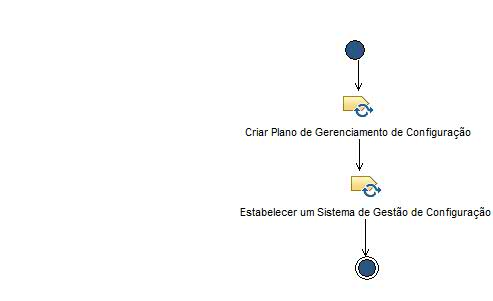
\includegraphics[scale=1.3]{./images/processonpi}
\label{fig:procnpi}
\legend {\fontsize{10}{12}\selectfont Fonte: \citeonline{processonpi}.}
\end{figure}


\chapter{Trabalhos Relacionados}\label{trabalhorel}
Nesta seção será descrito trabalhos que influenciaram os conceitos envolvidos neste trabalho além de demonstrar pontos comuns e distintos entre si e o proposto.

O trabalho de \citeonline{pereira2013} descreve a implantação de uma ferramenta de integração contínua em um departamento de desenvolvimento e pesquisa, o Sedna, de uma empresa de engenharia em um ambiente de MPS.BR nível F. Os principais clientes do Sedna são voltados a área de óleo e gás.

Durante o período de implantação, o Sedna fornecia manutenção a três sistemas, onde um tratava-se de uma aplicação web, deste modo o \textit{deploy} da aplicação para todos os seus usuários era de responsabilidade do Sedna. Tal ação tornava-se bastante custosa devido ao grande número de web sites que deveriam ser atualizados.
	
Dentro do Sedna algumas ferramentas de gerência de configuração já eram utilizadas, tais como o Atlassian Jira, Subversion (SVN) e o Atlassian Confluence. Ainda com a utilização destas ferramentas a equipe possuia grandes dificuldades no tempo de realização do \textit{deploy}, pois esta atividade consumia uma grande parte do tempo da equipe, tempo de aprendizagem e realização do \textit{deploy} da aplicação principalmente para novos membros da equipe e um \textit{feedback} atrasado para problemas básicos de commits errôneos.

Os autores descrevem que como pontos positivos da integração estão a utilização de uma ferramenta de integração contínua da mesma empresa que fornecia o sistema de gerenciamento de projetos, a ferramenta utilizada foi o Atlassian Bamboo e a utilização de ferramentas da automação do processo de build o que facilitava o trabalho da integração contínua. Bem como o autor destaca as experiências negativas da implantação, que estão na ausência de uma máquina com requisitos mínimos exigidos para a utilização, a ausência de treinamento da equipe, onde os conhecimentos de IC estava com o líder de projeto e o gerente de configuração e por fim a ferramenta não fornecia suporte ao \textit{redeploy} dos artefatos gerados, o que criou um barreira na equipe acerca da ferramenta.


\cite{abdul2012}

Uma das principiais vantagens da utilização da integração contínua é o seu \textit{feedback} imediato acerca de problemas de integração, e entender e interpretar as principais causas dos problemas de integração foi realizado por \citeonline{miller2008}. Quando este percebeu que em um projeto da Microsoft, o Service Factory, a maior causa de quebra de build eram violações no sistema de análise de código, seguido por testes automatizados e erros de compilação.

A coleta de métricas através da inspeção contínua é uma grande vantagem incluída dentro da Integração Contínua, pois a sua principal vantagem é aumentar a qualidade do produto e facilitar o processo de manutenção do software. Para isso \citeonline{moreira2010} desenvolveram um framework para extração de métricas de forma automatizada implementado em um ambiente de Integração Contínua, logo ficou evidente importância das inspeções e teste de códigos nas builds como foi descrito anteriormente.

Os testes por serem peça fundamental na qualidade no software e na confiança do produto, além de serem fundamentais em uma build de integração contínua, \citeonline{kim2009} propuseram a criação de um framework automatizado de testes que permitissem facilitar os casos de testes, reuso de componentes, relatórios mais legíveis e integrado com um ambiente de integração contínua.

%%% abtex2-modelo-include-comandos.tex, v-1.9.2 laurocesar
%% Copyright 2012-2014 by abnTeX2 group at http://abntex2.googlecode.com/ 
%%
%% This work may be distributed and/or modified under the
%% conditions of the LaTeX Project Public License, either version 1.3
%% of this license or (at your option) any later version.
%% The latest version of this license is in
%%   http://www.latex-project.org/lppl.txt
%% and version 1.3 or later is part of all distributions of LaTeX
%% version 2005/12/01 or later.
%%
%% This work has the LPPL maintenance status `maintained'.
%% 
%% The Current Maintainer of this work is the abnTeX2 team, led
%% by Lauro César Araujo. Further information are available on 
%% http://abntex2.googlecode.com/
%%
%% This work consists of the files abntex2-modelo-include-comandos.tex
%% and abntex2-modelo-img-marca.pdf
%%

% ---
% Este capítulo, utilizado por diferentes exemplos do abnTeX2, ilustra o uso de
% comandos do abnTeX2 e de LaTeX.
% ---
 
\chapter{Resultados de comandos}\label{cap_exemplos}

\chapterprecis{Isto é uma sinopse de capítulo. A ABNT não traz nenhuma
normatização a respeito desse tipo de resumo, que é mais comum em romances 
e livros técnicos.}\index{sinopse de capítulo}

% ---
\section{Codificação dos arquivos: UTF8}
% ---

A codificação de todos os arquivos do \abnTeX\ é \texttt{UTF8}. É necessário que
você utilize a mesma codificação nos documentos que escrever, inclusive nos
arquivos de base bibliográficas |.bib|.

% ---
\section{Citações diretas}
\label{sec-citacao}
% ---

\index{citações!diretas}Utilize o ambiente \texttt{citacao} para incluir
citações diretas com mais de três linhas:

\begin{citacao}
As citações diretas, no texto, com mais de três linhas, devem ser
destacadas com recuo de 4 cm da margem esquerda, com letra menor que a do texto
utilizado e sem as aspas. No caso de documentos datilografados, deve-se
observar apenas o recuo \cite[5.3]{NBR10520:2002}.
\end{citacao}

Use o ambiente assim:

\begin{verbatim}
\begin{citacao}
As citações diretas, no texto, com mais de três linhas [...] deve-se observar
apenas o recuo \cite[5.3]{NBR10520:2002}.
\end{citacao}
\end{verbatim}

O ambiente \texttt{citacao} pode receber como parâmetro opcional um nome de
idioma previamente carregado nas opções da classe (\autoref{sec-hifenizacao}). Nesse
caso, o texto da citação é automaticamente escrito em itálico e a hifenização é
ajustada para o idioma selecionado na opção do ambiente. Por exemplo:

\begin{verbatim}
\begin{citacao}[english]
Text in English language in italic with correct hyphenation.
\end{citacao}
\end{verbatim}

Tem como resultado:

\begin{citacao}[english]
Text in English language in italic with correct hyphenation.
\end{citacao}

\index{citações!simples}Citações simples, com até três linhas, devem ser
incluídas com aspas. Observe que em \LaTeX as aspas iniciais são diferentes das
finais: ``Amor é fogo que arde sem se ver''.

% ---
\section{Notas de rodapé}
% ---

As notas de rodapé são detalhadas pela NBR 14724:2011 na seção 5.2.1\footnote{As
notas devem ser digitadas ou datilografadas dentro das margens, ficando
separadas do texto por um espaço simples de entre as linhas e por filete de 5
cm, a partir da margem esquerda. Devem ser alinhadas, a partir da segunda linha
da mesma nota, abaixo da primeira letra da primeira palavra, de forma a destacar
o expoente, sem espaço entre elas e com fonte menor
\citeonline[5.2.1]{NBR14724:2011}.}\footnote{Caso uma série de notas sejam
criadas sequencialmente, o \abnTeX\ instrui o \LaTeX\ para que uma vírgula seja
colocada após cada número do expoente que indica a nota de rodapé no corpo do
texto.}\footnote{Verifique se os números do expoente possuem uma vírgula para
dividi-los no corpo do texto.}. 


% ---
\section{Tabelas}
% ---

\index{tabelas}A \autoref{tab-nivinv} é um exemplo de tabela construída em
\LaTeX.

\begin{table}[htb]
\ABNTEXfontereduzida
\caption[Níveis de investigação]{Níveis de investigação.}
\label{tab-nivinv}
\begin{tabular}{p{2.6cm}|p{6.0cm}|p{2.25cm}|p{3.40cm}}
  %\hline
   \textbf{Nível de Investigação} & \textbf{Insumos}  & \textbf{Sistemas de Investigação}  & \textbf{Produtos}  \\
    \hline
    Meta-nível & Filosofia\index{filosofia} da Ciência  & Epistemologia &
    Paradigma  \\
    \hline
    Nível do objeto & Paradigmas do metanível e evidências do nível inferior &
    Ciência  & Teorias e modelos \\
    \hline
    Nível inferior & Modelos e métodos do nível do objeto e problemas do nível inferior & Prática & Solução de problemas  \\
   % \hline
\end{tabular}
\legend{Fonte: \citeonline{van86}}
\end{table}

Já a \autoref{tabela-ibge} apresenta uma tabela criada conforme o padrão do
\citeonline{ibge1993} requerido pelas normas da ABNT para documentos técnicos e
acadêmicos.

\begin{table}[htb]
\IBGEtab{%
  \caption{Um Exemplo de tabela alinhada que pode ser longa
  ou curta, conforme padrão IBGE.}%
  \label{tabela-ibge}
}{%
  \begin{tabular}{ccc}
  \toprule
   Nome & Nascimento & Documento \\
  \midrule \midrule
   Maria da Silva & 11/11/1111 & 111.111.111-11 \\
  \midrule 
   João Souza & 11/11/2111 & 211.111.111-11 \\
  \midrule 
   Laura Vicuña & 05/04/1891 & 3111.111.111-11 \\
  \bottomrule
\end{tabular}%
}{%
  \fonte{Produzido pelos autores.}%
  \nota{Esta é uma nota, que diz que os dados são baseados na
  regressão linear.}%
  \nota[Anotações]{Uma anotação adicional, que pode ser seguida de várias
  outras.}%
  }
\end{table}


% ---
\section{Figuras}
% ---

\index{figuras}Figuras podem ser criadas diretamente em \LaTeX,
como o exemplo da \autoref{fig_circulo}.

\begin{figure}[htb]
	\caption{\label{fig_circulo}A delimitação do espaço}
	\begin{center}
	    \setlength{\unitlength}{5cm}
		\begin{picture}(1,1)
		\put(0,0){\line(0,1){1}}
		\put(0,0){\line(1,0){1}}
		\put(0,0){\line(1,1){1}}
		\put(0,0){\line(1,2){.5}}
		\put(0,0){\line(1,3){.3333}}
		\put(0,0){\line(1,4){.25}}
		\put(0,0){\line(1,5){.2}}
		\put(0,0){\line(1,6){.1667}}
		\put(0,0){\line(2,1){1}}
		\put(0,0){\line(2,3){.6667}}
		\put(0,0){\line(2,5){.4}}
		\put(0,0){\line(3,1){1}}
		\put(0,0){\line(3,2){1}}
		\put(0,0){\line(3,4){.75}}
		\put(0,0){\line(3,5){.6}}
		\put(0,0){\line(4,1){1}}
		\put(0,0){\line(4,3){1}}
		\put(0,0){\line(4,5){.8}}
		\put(0,0){\line(5,1){1}}
		\put(0,0){\line(5,2){1}}
		\put(0,0){\line(5,3){1}}
		\put(0,0){\line(5,4){1}}
		\put(0,0){\line(5,6){.8333}}
		\put(0,0){\line(6,1){1}}
		\put(0,0){\line(6,5){1}}
		\end{picture}
	\end{center}
	\legend{Fonte: os autores}
\end{figure}

Ou então figuras podem ser incorporadas de arquivos externos, como é o caso da
\autoref{fig_grafico}. Se a figura que ser incluída se tratar de um diagrama, um
gráfico ou uma ilustração que você mesmo produza, priorize o uso de imagens
vetoriais no formato PDF. Com isso, o tamanho do arquivo final do trabalho será
menor, e as imagens terão uma apresentação melhor, principalmente quando
impressas, uma vez que imagens vetorias são perfeitamente escaláveis para
qualquer dimensão. Nesse caso, se for utilizar o Microsoft Excel para produzir
gráficos, ou o Microsoft Word para produzir ilustrações, exporte-os como PDF e
os incorpore ao documento conforme o exemplo abaixo. No entanto, para manter a
coerência no uso de software livre (já que você está usando \LaTeX e \abnTeX),
teste a ferramenta \textsf{InkScape}\index{InkScape}
(\url{http://inkscape.org/}). Ela é uma excelente opção de código-livre para
produzir ilustrações vetoriais, similar ao CorelDraw\index{CorelDraw} ou ao Adobe
Illustrator\index{Adobe Illustrator}. De todo modo, caso não seja possível
utilizar arquivos de imagens como PDF, utilize qualquer outro formato, como
JPEG, GIF, BMP, etc. Nesse caso, você pode tentar aprimorar as imagens
incorporadas com o software livre \textsf{Gimp}\index{Gimp}
(\url{http://www.gimp.org/}). Ele é uma alternativa livre ao Adobe
Photoshop\index{Adobe Photoshop}.

\begin{figure}[htb]
	\caption{\label{fig_grafico}Gráfico produzido em Excel e salvo como PDF}
	\begin{center}
	    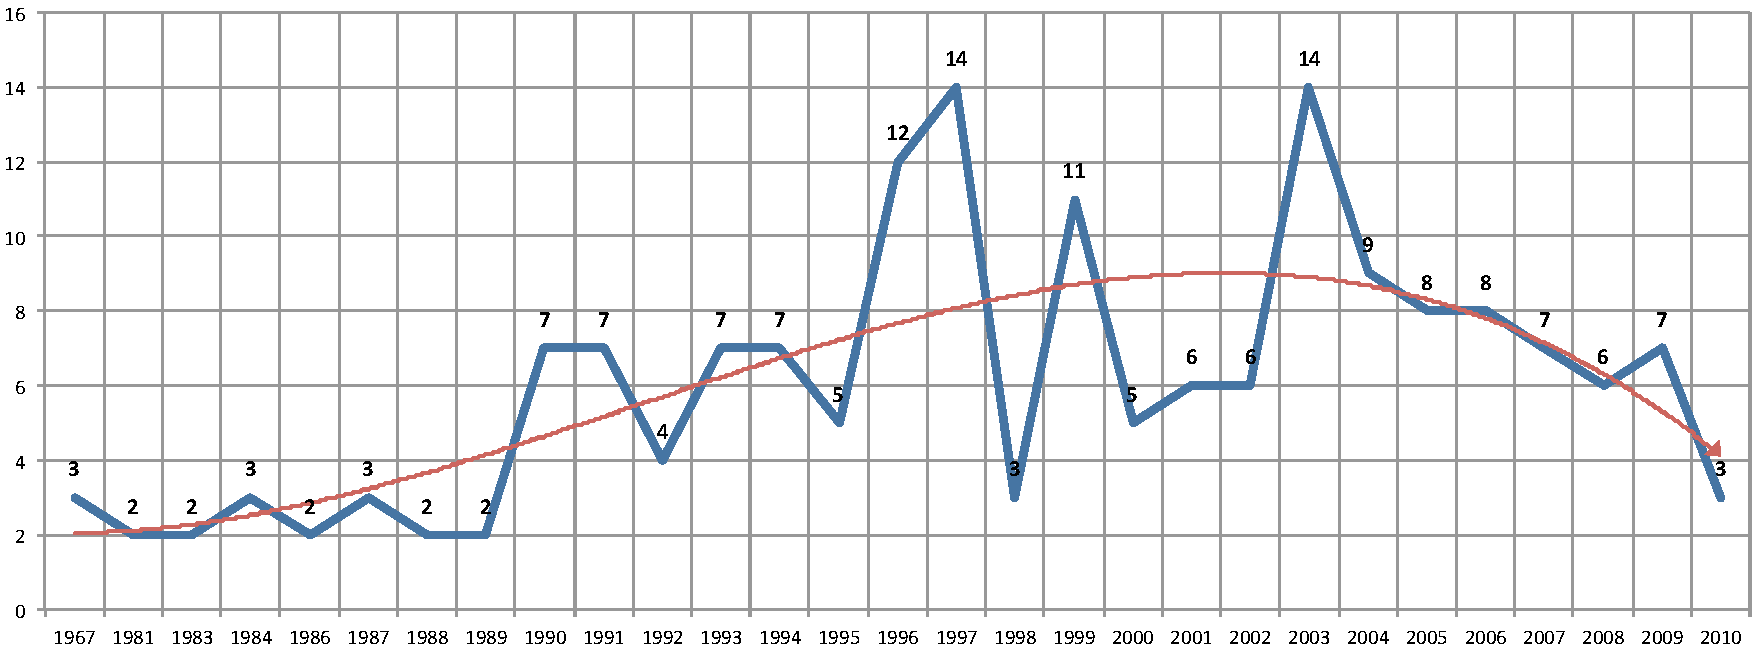
\includegraphics[scale=0.5]{abntex2-modelo-img-grafico.pdf}
	\end{center}
	\legend{Fonte: \citeonline[p. 24]{araujo2012}}
\end{figure}

% ---
\subsection{Figuras em \emph{minipages}}
% ---

\emph{Minipages} são usadas para inserir textos ou outros elementos em quadros
com tamanhos e posições controladas. Veja o exemplo da
\autoref{fig_minipage_imagem1} e da \autoref{fig_minipage_grafico2}.

\begin{figure}[htb]
 \label{teste}
 \centering
  \begin{minipage}{0.4\textwidth}
    \centering
    \caption{Imagem 1 da minipage} \label{fig_minipage_imagem1}
    
\includegraphics[scale=0.9]{abntex2-modelo-img-marca.pdf}
    \legend{Fonte: Produzido pelos autores}
  \end{minipage}
  \hfill
  \begin{minipage}{0.4\textwidth}
    \centering
    \caption{Grafico 2 da minipage} \label{fig_minipage_grafico2}
    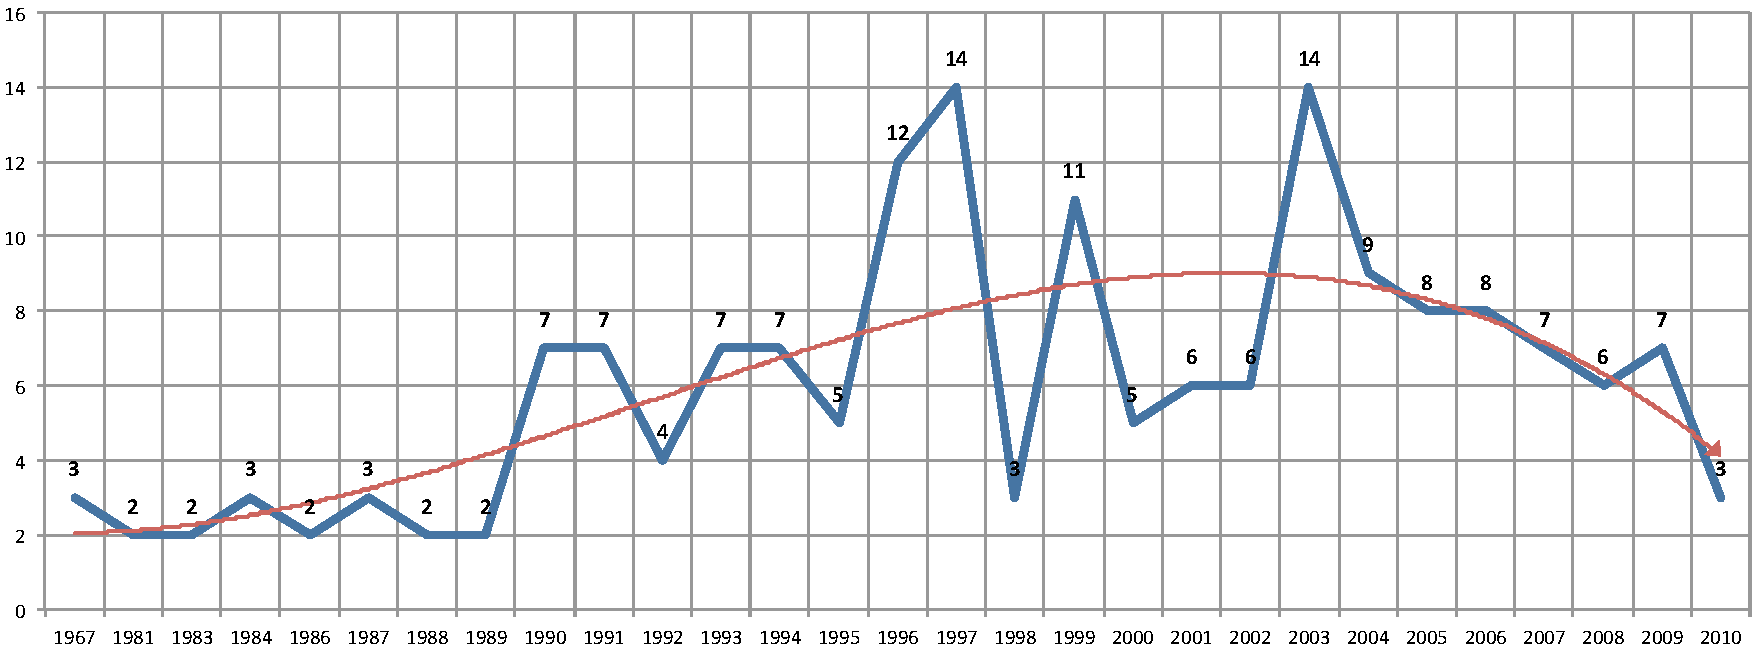
\includegraphics[scale=0.2]{abntex2-modelo-img-grafico.pdf}
    \legend{Fonte: \citeonline[p. 24]{araujo2012}}
  \end{minipage}
\end{figure}

Observe que, segundo a \citeonline[seções 4.2.1.10 e 5.8]{NBR14724:2011}, as
ilustrações devem sempre ter numeração contínua e única em todo o documento:

\begin{citacao}
Qualquer que seja o tipo de ilustração, sua identificação aparece na parte
superior, precedida da palavra designativa (desenho, esquema, fluxograma,
fotografia, gráfico, mapa, organograma, planta, quadro, retrato, figura,
imagem, entre outros), seguida de seu número de ordem de ocorrência no texto,
em algarismos arábicos, travessão e do respectivo título. Após a ilustração, na
parte inferior, indicar a fonte consultada (elemento obrigatório, mesmo que
seja produção do próprio autor), legenda, notas e outras informações
necessárias à sua compreensão (se houver). A ilustração deve ser citada no
texto e inserida o mais próximo possível do trecho a que se
refere. \cite[seções 5.8]{NBR14724:2011}
\end{citacao}

% ---
\section{Expressões matemáticas}
% ---

\index{expressões matemáticas}Use o ambiente \texttt{equation} para escrever
expressões matemáticas numeradas:

\begin{equation}
  \forall x \in X, \quad \exists \: y \leq \epsilon
\end{equation}

Escreva expressões matemáticas entre \$ e \$, como em $ \lim_{x \to \infty}
\exp(-x) = 0 $, para que fiquem na mesma linha.

Também é possível usar colchetes para indicar o início de uma expressão
matemática que não é numerada.

\[
\left|\sum_{i=1}^n a_ib_i\right|
\le
\left(\sum_{i=1}^n a_i^2\right)^{1/2}
\left(\sum_{i=1}^n b_i^2\right)^{1/2}
\]

Consulte mais informações sobre expressões matemáticas em
\url{https://code.google.com/p/abntex2/wiki/Referencias}.

% ---
\section{Enumerações: alíneas e subalíneas}
% ---

\index{alíneas}\index{subalíneas}\index{incisos}Quando for necessário enumerar
os diversos assuntos de uma seção que não possua título, esta deve ser
subdividida em alíneas \cite[4.2]{NBR6024:2012}:

\begin{alineas}

  \item os diversos assuntos que não possuam título próprio, dentro de uma mesma
  seção, devem ser subdivididos em alíneas; 
  
  \item o texto que antecede as alíneas termina em dois pontos;
  \item as alíneas devem ser indicadas alfabeticamente, em letra minúscula,
  seguida de parêntese. Utilizam-se letras dobradas, quando esgotadas as
  letras do alfabeto;

  \item as letras indicativas das alíneas devem apresentar recuo em relação à
  margem esquerda;

  \item o texto da alínea deve começar por letra minúscula e terminar em
  ponto-e-vírgula, exceto a última alínea que termina em ponto final;

  \item o texto da alínea deve terminar em dois pontos, se houver subalínea;

  \item a segunda e as seguintes linhas do texto da alínea começa sob a
  primeira letra do texto da própria alínea;
  
  \item subalíneas \cite[4.3]{NBR6024:2012} devem ser conforme as alíneas a
  seguir:

  \begin{alineas}
     \item as subalíneas devem começar por travessão seguido de espaço;

     \item as subalíneas devem apresentar recuo em relação à alínea;

     \item o texto da subalínea deve começar por letra minúscula e terminar em
     ponto-e-vírgula. A última subalínea deve terminar em ponto final, se não
     houver alínea subsequente;

     \item a segunda e as seguintes linhas do texto da subalínea começam sob a
     primeira letra do texto da própria subalínea.
  \end{alineas}
  
  \item no \abnTeX\ estão disponíveis os ambientes \texttt{incisos} e
  \texttt{subalineas}, que em suma são o mesmo que se criar outro nível de
  \texttt{alineas}, como nos exemplos à seguir:
  
  \begin{incisos}
    \item \textit{Um novo inciso em itálico};
  \end{incisos}
  
  \item Alínea em \textbf{negrito}:
  
  \begin{subalineas}
    \item \textit{Uma subalínea em itálico};
    \item \underline{\textit{Uma subalínea em itálico e sublinhado}}; 
  \end{subalineas}
  
  \item Última alínea com \emph{ênfase}.
  
\end{alineas}

% ---
\section{Espaçamento entre parágrafos e linhas}
% ---

\index{espaçamento!dos parágrafos}O tamanho do parágrafo, espaço entre a margem
e o início da frase do parágrafo, é definido por:

\begin{verbatim}
   \setlength{\parindent}{1.3cm}
\end{verbatim}

\index{espaçamento!do primeiro parágrafo}Por padrão, não há espaçamento no
primeiro parágrafo de cada início de divisão do documento
(\autoref{sec-divisoes}). Porém, você pode definir que o primeiro parágrafo
também seja indentado, como é o caso deste documento. Para isso, apenas inclua o
pacote \textsf{indentfirst} no preâmbulo do documento:

\begin{verbatim}
   \usepackage{indentfirst}      % Indenta o primeiro parágrafo de cada seção.
\end{verbatim}

\index{espaçamento!entre os parágrafos}O espaçamento entre um parágrafo e outro
pode ser controlado por meio do comando:

\begin{verbatim}
  \setlength{\parskip}{0.2cm}  % tente também \onelineskip
\end{verbatim}

\index{espaçamento!entre as linhas}O controle do espaçamento entre linhas é
definido por:

\begin{verbatim}
  \OnehalfSpacing       % espaçamento um e meio (padrão); 
  \DoubleSpacing        % espaçamento duplo
  \SingleSpacing        % espaçamento simples	
\end{verbatim}

Para isso, também estão disponíveis os ambientes:

\begin{verbatim}
  \begin{SingleSpace} ...\end{SingleSpace}
  \begin{Spacing}{hfactori} ... \end{Spacing}
  \begin{OnehalfSpace} ... \end{OnehalfSpace}
  \begin{OnehalfSpace*} ... \end{OnehalfSpace*}
  \begin{DoubleSpace} ... \end{DoubleSpace}
  \begin{DoubleSpace*} ... \end{DoubleSpace*} 
\end{verbatim}

Para mais informações, consulte \citeonline[p. 47-52 e 135]{memoir}.

% ---
\section{Inclusão de outros arquivos}\label{sec-include}
% ---

É uma boa prática dividir o seu documento em diversos arquivos, e não
apenas escrever tudo em um único. Esse recurso foi utilizado neste
documento. Para incluir diferentes arquivos em um arquivo principal,
de modo que cada arquivo incluído fique em uma página diferente, utilize o
comando:

\begin{verbatim}
   \include{documento-a-ser-incluido}      % sem a extensão .tex
\end{verbatim}

Para incluir documentos sem quebra de páginas, utilize:

\begin{verbatim}
   \input{documento-a-ser-incluido}      % sem a extensão .tex
\end{verbatim}

% ---
\section{Compilar o documento \LaTeX}
% ---

Geralmente os editores \LaTeX, como o
TeXlipse\footnote{\url{http://texlipse.sourceforge.net/}}, o
Texmaker\footnote{\url{http://www.xm1math.net/texmaker/}}, entre outros,
compilam os documentos automaticamente, de modo que você não precisa se
preocupar com isso.

No entanto, você pode compilar os documentos \LaTeX usando os seguintes
comandos, que devem ser digitados no \emph{Prompt de Comandos} do Windows ou no
\emph{Terminal} do Mac ou do Linux:

\begin{verbatim}
   pdflatex ARQUIVO_PRINCIPAL.tex
   bibtex ARQUIVO_PRINCIPAL.aux
   makeindex ARQUIVO_PRINCIPAL.idx 
   makeindex ARQUIVO_PRINCIPAL.nlo -s nomencl.ist -o ARQUIVO_PRINCIPAL.nls
   pdflatex ARQUIVO_PRINCIPAL.tex
   pdflatex ARQUIVO_PRINCIPAL.tex
\end{verbatim}

% ---
\section{Remissões internas}
% ---

Ao nomear a \autoref{tab-nivinv} e a \autoref{fig_circulo}, apresentamos um
exemplo de remissão interna, que também pode ser feita quando indicamos o
\autoref{cap_exemplos}, que tem o nome \emph{\nameref{cap_exemplos}}. O número
do capítulo indicado é \ref{cap_exemplos}, que se inicia à
\autopageref{cap_exemplos}\footnote{O número da página de uma remissão pode ser
obtida também assim:
\pageref{cap_exemplos}.}.
Veja a \autoref{sec-divisoes} para outros exemplos de remissões internas entre
seções, subseções e subsubseções.

O código usado para produzir o texto desta seção é:

\begin{verbatim}
Ao nomear a \autoref{tab-nivinv} e a \autoref{fig_circulo}, apresentamos um
exemplo de remissão interna, que também pode ser feita quando indicamos o
\autoref{cap_exemplos}, que tem o nome \emph{\nameref{cap_exemplos}}. O número
do capítulo indicado é \ref{cap_exemplos}, que se inicia à
\autopageref{cap_exemplos}\footnote{O número da página de uma remissão pode ser
obtida também assim:
\pageref{cap_exemplos}.}.
Veja a \autoref{sec-divisoes} para outros exemplos de remissões internas entre
seções, subseções e subsubseções.
\end{verbatim}

% ---
\section{Divisões do documento: seção}\label{sec-divisoes}
% ---

Esta seção testa o uso de divisões de documentos. Esta é a
\autoref{sec-divisoes}. Veja a \autoref{sec-divisoes-subsection}.

\subsection{Divisões do documento: subseção}\label{sec-divisoes-subsection}

Isto é uma subseção. Veja a \autoref{sec-divisoes-subsubsection}, que é uma
\texttt{subsubsection} do \LaTeX, mas é impressa chamada de ``subseção'' porque
no Português não temos a palavra ``subsubseção''.

\subsubsection{Divisões do documento: subsubseção}
\label{sec-divisoes-subsubsection}

Isto é uma subsubseção.

\subsubsection{Divisões do documento: subsubseção}

Isto é outra subsubseção.

\subsection{Divisões do documento: subseção}\label{sec-exemplo-subsec}

Isto é uma subseção.

\subsubsection{Divisões do documento: subsubseção}

Isto é mais uma subsubseção da \autoref{sec-exemplo-subsec}.


\subsubsubsection{Esta é uma subseção de quinto nível}\label{sec-exemplo-subsubsubsection}

Esta é uma seção de quinto nível. Ela é produzida com o seguinte comando:

\begin{verbatim}
\subsubsubsection{Esta é uma subseção de quinto
nível}\label{sec-exemplo-subsubsubsection}
\end{verbatim}

\subsubsubsection{Esta é outra subseção de quinto nível}\label{sec-exemplo-subsubsubsection-outro}

Esta é outra seção de quinto nível.


\paragraph{Este é um parágrafo numerado}\label{sec-exemplo-paragrafo}

Este é um exemplo de parágrafo nomeado. Ele é produzida com o comando de
parágrafo:

\begin{verbatim}
\paragraph{Este é um parágrafo nomeado}\label{sec-exemplo-paragrafo}
\end{verbatim}

A numeração entre parágrafos numeradaos e subsubsubseções são contínuas.

\paragraph{Esta é outro parágrafo numerado}\label{sec-exemplo-paragrafo-outro}

Esta é outro parágrafo nomeado.

% ---
\section{Este é um exemplo de nome de seção longo. Ele deve estar
alinhado à esquerda e a segunda e demais linhas devem iniciar logo abaixo da
primeira palavra da primeira linha}
% ---

Isso atende à norma \citeonline[seções de 5.2.2 a 5.2.4]{NBR14724:2011} 
 e \citeonline[seções de 3.1 a 3.8]{NBR6024:2012}.

% ---
\section{Diferentes idiomas e hifenizações}
\label{sec-hifenizacao}
% ---

Para usar hifenizações de diferentes idiomas, inclua nas opções do documento o
nome dos idiomas que o seu texto contém. Por exemplo (para melhor
visualização, as opções foram quebras em diferentes linhas):

\begin{verbatim}
\documentclass[
	12pt,
	openright,
	twoside,
	a4paper,
	english,
	french,
	spanish,
	brazil
	]{abntex2}
\end{verbatim}

O idioma português-brasileiro (\texttt{brazil}) é incluído automaticamente pela
classe \textsf{abntex2}. Porém, mesmo assim a opção \texttt{brazil} deve ser
informada como a última opção da classe para que todos os pacotes reconheçam o
idioma. Vale ressaltar que a última opção de idioma é a utilizada por padrão no
documento. Desse modo, caso deseje escrever um texto em inglês que tenha
citações em português e em francês, você deveria usar o preâmbulo como abaixo:

\begin{verbatim}
\documentclass[
	12pt,
	openright,
	twoside,
	a4paper,
	french,
	brazil,
	english
	]{abntex2}
\end{verbatim}

A lista completa de idiomas suportados, bem como outras opções de hifenização,
estão disponíveis em \citeonline[p.~5-6]{babel}.

Exemplo de hifenização em inglês\footnote{Extraído de:
\url{http://en.wikibooks.org/wiki/LaTeX/Internationalization}}:

\begin{otherlanguage*}{english}
\textit{Text in English language. This environment switches all language-related
definitions, like the language specific names for figures, tables etc. to the other
language. The starred version of this environment typesets the main text
according to the rules of the other language, but keeps the language specific
string for ancillary things like figures, in the main language of the document.
The environment hyphenrules switches only the hyphenation patterns used; it can
also be used to disallow hyphenation by using the language name
`nohyphenation'.}
\end{otherlanguage*}

Exemplo de hifenização em francês\footnote{Extraído de:
\url{http://bigbrowser.blog.lemonde.fr/2013/02/17/tu-ne-tweeteras-point-le-vatican-interdit-aux-cardinaux-de-tweeter-pendant-le-conclave/}}:

\begin{otherlanguage*}{french}
\textit{Texte en français. Pas question que Twitter ne vienne faire une
concurrence déloyale à la traditionnelle fumée blanche qui marque l'élection
d'un nouveau pape. Pour éviter toute fuite précoce, le Vatican a donc pris un
peu d'avance, et a déjà interdit aux cardinaux qui prendront part au vote
d'utiliser le réseau social, selon Catholic News Service. Une mesure valable
surtout pour les neuf cardinaux – sur les 117 du conclave – pratiquants très
actifs de Twitter, qui auront interdiction pendant toute la période de se
connecter à leur compte.}
\end{otherlanguage*}

Pequeno texto em espanhol\footnote{Extraído de:
\url{http://internacional.elpais.com/internacional/2013/02/17/actualidad/1361102009_913423.html}}:

\foreignlanguage{spanish}{\textit{Decenas de miles de personas ovacionan al pontífice en su
penúltimo ángelus dominical, el primero desde que anunciase su renuncia. El Papa se
centra en la crítica al materialismo}}.

O idioma geral do texto por ser alterado como no exemplo seguinte:

\begin{verbatim}
  \selectlanguage{english}
\end{verbatim}

Isso altera automaticamente a hifenização e todos os nomes constantes de
referências do documento para o idioma inglês. Consulte o manual da classe
\cite{abntex2classe} para obter orientações adicionais sobre internacionalização de
documentos produzidos com \abnTeX.

A \autoref{sec-citacao} descreve o ambiente \texttt{citacao} que pode receber
como parâmetro um idioma a ser usado na citação.

% ---
\section{Consulte o manual da classe \textsf{abntex2}}
% ---

Consulte o manual da classe \textsf{abntex2} \cite{abntex2classe} para uma
referência completa das macros e ambientes disponíveis. 

Além disso, o manual possui informações adicionais sobre as normas ABNT
observadas pelo \abnTeX\ e considerações sobre eventuais requisitos específicos
não atendidos, como o caso da \citeonline[seção 5.2.2]{NBR14724:2011}, que
especifica o espaçamento entre os capítulos e o início do texto, regra
propositalmente não atendida pelo presente modelo.

% ---
\section{Referências bibliográficas}
% ---

A formatação das referências bibliográficas conforme as regras da ABNT são um
dos principais objetivos do \abnTeX. Consulte os manuais
\citeonline{abntex2cite} e \citeonline{abntex2cite-alf} para obter informações
sobre como utilizar as referências bibliográficas.

%-
\subsection{Acentuação de referências bibliográficas}
%-

Normalmente não há problemas em usar caracteres acentuados em arquivos
bibliográficos (\texttt{*.bib}). Porém, como as regras da ABNT fazem uso quase
abusivo da conversão para letras maiúsculas, é preciso observar o modo como se
escreve os nomes dos autores. Na ~\autoref{tabela-acentos} você encontra alguns
exemplos das conversões mais importantes. Preste atenção especial para `ç' e `í'
que devem estar envoltos em chaves. A regra geral é sempre usar a acentuação
neste modo quando houver conversão para letras maiúsculas.

\begin{table}[htbp]
\caption{Tabela de conversão de acentuação.}
\label{tabela-acentos}

\begin{center}
\begin{tabular}{ll}\hline\hline
acento & \textsf{bibtex}\\
à á ã & \verb+\`a+ \verb+\'a+ \verb+\~a+\\
í & \verb+{\'\i}+\\
ç & \verb+{\c c}+\\
\hline\hline
\end{tabular}
\end{center}
\end{table}


% ---
\section{Precisa de ajuda?}
% ---

Consulte a FAQ com perguntas frequentes e comuns no portal do \abnTeX:
\url{https://code.google.com/p/abntex2/wiki/FAQ}.

Inscreva-se no grupo de usuários \LaTeX:
\url{http://groups.google.com/group/latex-br}, tire suas dúvidas e ajude
outros usuários.

Participe também do grupo de desenvolvedores do \abnTeX:
\url{http://groups.google.com/group/abntex2} e faça sua contribuição à
ferramenta.

% ---
\section{Você pode ajudar?}
% ---

Sua contribuição é muito importante! Você pode ajudar na divulgação, no
desenvolvimento e de várias outras formas. Veja como contribuir com o \abnTeX\
em \url{https://code.google.com/p/abntex2/wiki/ComoContribuir}.

% ---
\section{Quer customizar os modelos do \abnTeX\ para sua instituição ou
universidade?}
% ---

Veja como customizar o \abnTeX\ em:
\url{https://code.google.com/p/abntex2/wiki/ComoCustomizar}.


%\chapter{Objetivos}\label{objetivos}
\section{Objetivo Geral}\label{objetivoger}
Implantar uma ferramenta de integração contínua no Núcleo de Práticas em Informática da Universidade Federal do Ceará do campus Quixadá.

\section{Objetivos Específicos}

\begin{itemize}
\item Estudar e analisar ferramentas de integração contínua e selecionar a que melhor se adapta ao Núcleo de Práticas em Informática;
\item Selecionar e implantar uma ferramenta de integração contínua automatizada;
\item Coletar relatos e resultados provenientes da implantação da ferramenta.
\end{itemize}
% ----------------------------------------------------------
% PARTE II
% ----------------------------------------------------------
%\part{Referenciais Teóricos}


% Capitulo de revisão de literatura
%\chapter{Lorem ipsum dolor sit amet}
\chapter{Procedimentos Metodológicos}\label{metodologia}

\section{Analisar as atividades do Núcleo de Práticas}
Esta atividade visa identificar como as atividades ocorrem dentro do Núcleo de Práticas em Informática, para tal foi analisado o processo\footnote{www.npi.quixada.ufc.br/processo/} existente modelado pela ferramenta \textit{EPF Composer}. Além da experiência do autor, pois este era um estagiário da organização com experiência de 8 meses nas atividades lá realizadas. 

\section{Pesquisar e selecionar a ferramenta de Integração Contínua}

Esta atividade consiste em  colher informações e selecionar a ferramenta que melhor se adapta a realidade existente no Núcleo de Práticas em Informática. 
Para a escolha da ferramenta foi preciso definir um conjunto de requisitos que a ferramenta deveria possuir e suprir, de modo a filtrar a ferramenta escolhida dentre as diversas existentes. As definições foram descritas \autoref{escolhaFerramenta}. 

\section{Absorção do perfil dos estagiários do Núcleo de Práticas}
Esta atividade tem como objetivo entender e identificar os conhecimentos dos estagiários do núcleo acerca de integração contínua, experiência de uso em projetos pessoais, conhecimento na ferramenta e como esta funciona. Para tal fora realizado um questionário online de escopo fechado que tinha como objetivo extrair o conhecimentos dos estagiários sobre integração contínua, seu uso e gerência de configuração de software.

\section{Implantação da ferramenta de integração contínua}
A implantação será realizada no núcleo de práticas e a utilização da ferramenta será aplicada a um projeto piloto. Ao inicio será realizado um treinamento para explanação do funcionamento da ferramenta, bem como a utilização desta impactará nas atividades dos estagiários.

\section{Coleta de Métricas de Código}
Esta etapa consiste na coleta contínua de métricas através da inspeção contínua de código do software em desenvolvimento através da integração contínua. Para isso fora utilizado uma ferramenta de análise estática de código, o Sonarqube \footnote{www.sonarqube.org/} integrado ao Jenkins em um processo \textit{post-build}, que servirá de insumo para melhorias no código, afim de aumentar sua qualidade e diminuir esforços futuros de manutenção. 



% ----------------------------------------------------------
% PARTE III
% ----------------------------------------------------------
%\part{Resultados}
\chapter{Desenvolvimento/Resultados}
Esta seção tem como objetivo apresentar as etapas para a elaboração deste trabalho. A seção é composta de cinco subseções. A \autoref{Analise-NPI} retrata a primeira fase do trabalho onde é explanado as atividades do NPI. A \autoref{pesq-selecao} descreve como a ferramenta de integração contínua foi escolhida e sob quais critérios, enquanto que a \autoref{perfil-estagiarios} detalha qual é o perfil dos estagiários do NPI no que concede à integração contínua.


\section{Análise das atividades do Núcleo de Práticas em Informática}\label{Analise-NPI}
A análise de como as atividades eram executadas dentro do NPI foi primeiramente analisada de acordo com o processo definido, disponível no site do NPI \footnote{www.npi.quixada.ufc.br/processo/}, o qual regula como as atividades ocorrem. As atividades e o processo baseia-se no SCRUM e nas metodologias ágeis como equipes de pequeno número de componentes \textit{Sprint Planning}, \textit{Product Backlog}, \textit{Sprint Review}.

O NPI subdivide-se em dois turnos, manhã e tarde, sendo cada turno supervisionado por um professor orientador diferente. Estes turnos podem ou não estar trabalhando no mesmo projeto, embora o mais comum é que trabalhem em projetos diferentes. As equipes contam com em média oito membros onde comumente destes, dois são alocados para as atividades de requisitos e testes, um para liderança técnica, enquanto o restante da equipe é alocado para as atividades de desenvolvimento, incluindo o líder técnico. O professor supervisor tem como papel o auxílio aos líderes técnicos, acompanhamento do projeto, avaliação dos estagiários, escolha dos projetos a serem desenvolvidos pelas equipes e usualmente realizar o papel de \textit{Product Owner}. 

O líder técnico possui papel gerencial bem como de desenvolvimento, sua atribuições partem desde a condução de reuniões, resolução de conflitos,atribuição e definições de tarefas, até o acompanhamento das atividades. 

A \autoref{fig:processo-npi} mostra o processo utilizado no NPI modelado através da ferramenta EPF Composer. Na figura	existem duas atividades que ocorrem em paralelo, são elas: Avaliação do Processo e Iniciar Projeto, este que subdividi-se em mais três atividades, a primeira delas a atividade de Requisitos, que posteriormente fornece entrada para um ciclo de \textit{Sprints} que ocorrerá enquanto houver funcionalidades não implementadas, simultaneamente com a atividade de Requisitos estão de Gerenciamento do Projeto e o Gerenciamento de Configuração.
\begin{figure}[H]
\centering
\caption[Processo do NPI]{Processo do NPI.}
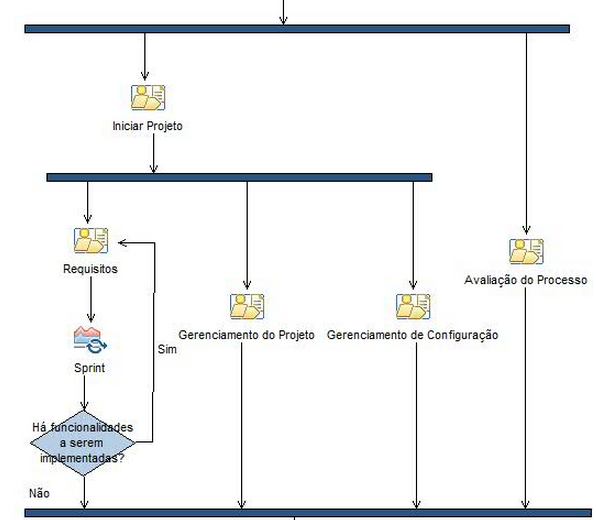
\includegraphics[scale=0.8]{./images/processo-npi}
\label{fig:processo-npi}
\legend {\fontsize{10}{12}\selectfont {Fonte: \citeonline{processonpi}}.}
\end{figure}

\section{Pesquisa e Seleção da Ferramenta}\label{pesq-selecao}
O processo de escolha da ferramenta de integração contínua teve como primeiro critério estar em acordo com a realidade das atividades executadas no NPI. Consequentemente o primeiro ponto a ser considerado foi o suporte que a ferramenta deveria prover as linguagens utilizadas no NPI, a linguagem Java. Outro aspecto considerado está relacionado com o custo de aquisição, esta não poderia ser paga ou deveria possuir uma versão \textit{free} que atendesse a demanda das atividades. Extensibilidade, devido as constantes mudanças de tecnologias utilizadas, fornecer suporte a diferentes linguagens, ferramentas, faz-se essencial; usabilidade, pois o NPI não conta com um Gerente de Configuração, sendo assim esta tarefa de manter uma integração contínua deve ser facilitada ao máximo por meio de sua usabilidade, tais como, \textit{inteligibilidade}, \textit{apreensibilidade}; possuir segurança adequada, definição de usuário, papéis.

Deste modo a ferramenta escolhida foi o Jenkins , anteriormente conhecido como Hudson, é uma ferramenta de integração contínua \textit{open source}, que fornece suporte a projetos de diferentes linguagens e tecnologias ,.NET, Ruby, Grails, PHP, bem como Java, linguagem base de sua construção. \cite{smart2011}, e como esta preenche os requisitos definidos será descrito abaixo.

\begin{itemize}
\item {\textbf{Suporte a Linguagem:}}

O Jenkins permite suporte a uma grande gama de linguagens, tais como Java, PHP, Rails, Grails, Python, entre outras.

\item {\textbf{Suporte ao Sistema de Controle de Versão:}}
O Jenkins consegue integrar nativamente com os principais sistemas de controle de versão tais como: \textit{CVS}, \textit{SVN},  \textit{Mercurial}, e o \textit{Git} através da utilização de plugin.


\item {\textbf{Segurança:}}
A segurança do Jenkins é habilitada através de permissões e papéis, onde a base de dados de usuários pode ser pela base interna do Jenkins, LDAP, usuários do sistema operacional e também através do usuário vinculado ao GitHub.

\item {\textbf{Extensibilidade:}}
Jenkins é extremamente flexível e adaptável, permitindo assim oferecer uma melhor atuação para diferentes propósitos, através das centenas de plugins disponíveis. Plugins este que oferecem tudo desde sistemas de controle de versão, ferramentas de build, ferramentas de análise estática de código, notificadores de build, alterações de UI, integração com sistemas externos (\textit{Jira, Redmine}) \cite{smart2011}.


\item {\textbf{Usabilidade:}}
"Primeiramente, Jenkins é fácil de usar. A interface é simples e intuitiva, e o Jenkins como um todo possui uma curva de aprendizado baixa"\space \cite[p~.3]{smart2011}.

\item {\textbf{Instalação e Configuração:}}

Facilidade de instalação, diferentes ambiente de operação, tais como sistemas operacionais, utilização de recursos. Documentação clara e objetiva do processo de instalação informando dependência existentes.

\end{itemize}

\section{Perfil dos Estagiários e conhecimentos sobre Integração Contínua}\label{perfil-estagiarios}
Entender os conhecimentos dos estagiários do NPI acerca do entendimento, funcionalidade e como esta mudaria suas rotinas de trabalho foi essencial para um entendimento e aperfeiçoamento do processo de implantação da ferramenta.

Para tal, fora realizado um questionário fechado, distribuído de maneira eletrônica para todos os estagiários do NPI. Embora todos não tenham respondido, uma boa amostra foi obtida em confronto com o número total de estagiários em atividade. O referido questionário será apresentado abaixo.

\pagebreak
\begin{table}[htb]
\centering
\caption[Conhecimentos em Integração Contínua]{Conhecimento em Integração Contínua.}
\label{tab-ic}
\begin{tabular}{p{5.0cm}l|p{5.0cm}|p{5.40cm}|p{5.40cm}}
  \hline
   \textbf{Perguntas} & \textbf{Opções de Respostas}\\
    \hline
    & Testador \\
    Qual a sua função no NPI? & Engenheiro de Requisitos \\
    & Testador \\
    & Líder Técnico / Gerente \\
    \hline
    Você sabe o que é Integração Contínua? & Sim \\
    & Não \\
    \hline
    Você já utilizou Integração Contínua em algum projeto? & Sim \\
    & Não \\
    \hline
    Você conhece ou utilizou alguma destas ferramentas de Integração Contínua?  & \\
    & Atlassian Bamboo \\
    & Apache Continuum \\
    & CruiseControl \\
    & Jenkins / Hudson \\
    & Outra \\
    & Desconheço ou nunca utilizei nenhuma delas \\
	\hline
	Você sabe o que é Gerência de Configuração? & Sim \\
	& Não \\
	\hline
\end{tabular}
\legend {\fontsize{10}{12}\selectfont {Fonte: Elaborado pelo autor}.}
\end{table}

Ao todo, vinte e três estagiários participaram da pesquisa, quase o NPI em sua totalidade, as devidas respostas serão exibidas abaixo na ordem em que as perguntas foram apresentadas aos questionados. A elaboração deste questionário teve como objetivo gerar dados quantitativos de modo a entender o perfil dos estagiários do NPI, facilitando assim o processo de implantação da ferramenta de integração contínua. Onde esses dados geraram conhecimentos para apresentação e explicação as equipes de forma mais proveitosa e focada nas dificuldades.


\begin{figure}[H]
\centering
\caption[Função NPI]{Função no NPI.}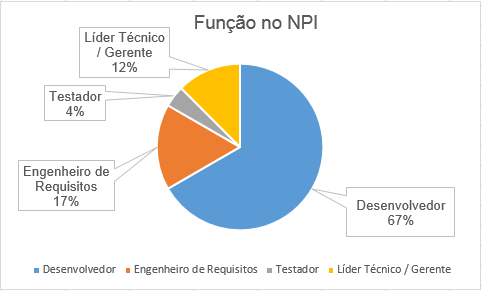
\includegraphics[scale=0.9]{./images/grafico-ci01}
\label{fig:grafico01-npi}
\legend {\fontsize{10}{12}\selectfont {Fonte: Elaborado pelo autor}.}
\end{figure}

A \autoref{fig:grafico01-npi} demonstra que a grande maioria dos estagiários do NPI estão alocados para atividades exclusivas de desenvolvimento, posteriormente atividade de engenharia de requisitos, líderes técnicos e gerentes. Este resultado obtido por meio das respostas ajudou a elucidar os conhecimentos e os tipos de conhecimentos predominante nos estagiários do núcleo.

\begin{figure}[H]
\centering
\caption[Conhecem Integração Contínua]{Conhecem Integração Contínua.}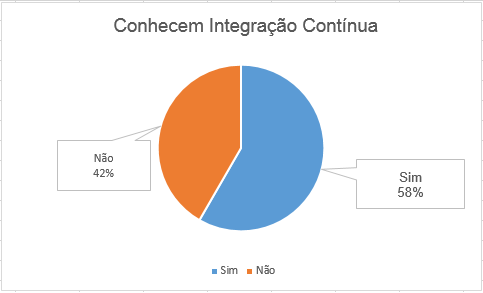
\includegraphics[scale=0.9]{./images/grafico-ci02}
\label{fig:grafico02-npi}
\legend {\fontsize{10}{12}\selectfont {Fonte: Elaborado pelo autor}.}
\end{figure}

Como descrito na \autoref{fig:grafico02-npi}, a maioria dos questionados conheciam o que era uma ferramenta de integração contínua, e como esta funcionava, embora esta não tenha sido uma superioridade notável, facilitou o processo de implantação em razão dos conhecimentos prévios dos estagiários a cerca do assunto, permitindo assim uma menor rejeição na implantação devido ao conhecimentos dos benefícios que este tipo de ferramenta causaria ao projeto.

\begin{figure}[H]
\centering
\caption[Utilização em Projetos Pessoais]{Utilização em Projetos Pessoais.}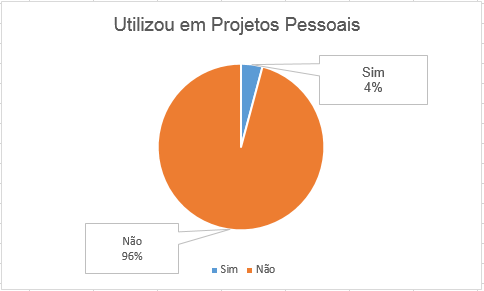
\includegraphics[scale=0.9]{./images/grafico-ci03}
\label{fig:grafico03-npi}
\legend {\fontsize{10}{12}\selectfont {Fonte: Elaborado pelo autor}.}
\end{figure}

Embora a maioria dos estagiários conheça a ferramenta, pouco mais de 4\% dos questionados utilizaram a integração contínua de forma prática, isto é, enfrentaram o impacto de sua utilização. Seja através do \textit{feedback} imediato fornecido pela ferramenta, ou pela alteração de seus processos de trabalho.	

\begin{figure}[H]
\centering
\caption[Conhecimento e Utilização de Ferramentas de Integração Contínua]{Conhecimento e Utilização de Ferramentas de Integração Contínua.}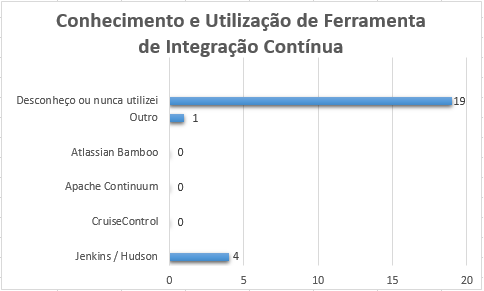
\includegraphics[scale=0.9]{./images/grafico-ci04}
\label{fig:grafico04-npi}
\legend {\fontsize{10}{12}\selectfont {Fonte: Elaborado pelo autor}.}
\end{figure}
O gráfico da \autoref{fig:grafico04-npi} contrasta com o gráfico anterior, onde a maioria desconhece ou nunca utilizou nenhuma ferramenta, e dentre a única ferramenta citada, o Jenkins / Hudson, enquanto um questionado citou outra ferramenta mas não especificou qual seria esta. De todo modo a familiarização de alguns questionados com a ferramenta facilitará o processo de aceitação desta por parte dos membros, e gerará uma unificação de conhecimento, pois todos os membros irão trabalhar e conhecer apenas uma ferramenta, no caso o Jenkins.

 

\begin{figure}[H]
\centering 
\caption[Conhecem Gerência de Configuração]{Conhecem Gerência de Configuração.}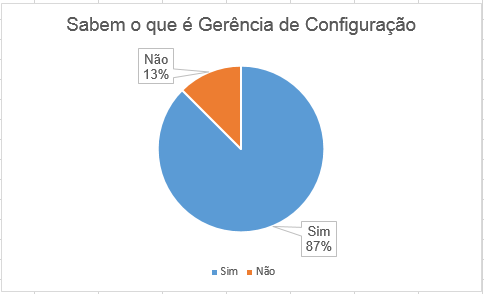
\includegraphics[scale=0.9]{./images/grafico-ci05}
\label{fig:grafico05-npi}
\legend {\fontsize{10}{12}\selectfont {Fonte: Elaborado pelo autor}.}
\end{figure}



\section{Processo de Implantação da Ferramenta de Integração Contínua}
Esta atividade tem como objetivo explicar como o processo ocorreu, apresentando o contexto do projeto, pontos negativos e positivos da implantação e aspectos a serem melhorados. A distribuição do conteúdo se dará da seguinte forma: \autoref{gpa} apresentará o projeto piloto onde a ferramenta foi implantada.


\subsection{Gestão de Projetos Acadêmicos }\label{gpa}
O projeto GPA (Gestão de Projetos Acadêmico) módulo de pesquisa tem como objetivo facilitar o processo de criação, submissão, aceitação e divulgação dos projetos da UFC do campus de Quixadá. Antes do desenvolvimento do sistema, este processo era totalmente manual. Enquanto este trabalho estava sendo desenvolvido o software do GPA era construído. Abaixo será descrito características deste sistema.

\begin{itemize}
	\item \textbf{Back-end:} A linguagem base da construção do sistema é o Java, com a utilização do Spring Framework. Este framework utiliza-se do padrão arquitetural MVC (Model View Control) além da rapidez de execução e segurança através da utilização do módulo de segurança Spring Security. A utilização do framework começou junto com a construção do sistema, sendo necessário treinamento aos membros das equipes, pois tratava-se de uma tecnologia nova no NPI.
	
	\item \textbf{Front-end:} Para a criação da aplicação front-end fora utilizado JSP (JavaServer Pages), HTML (HyperText Markup Language), CSS (Cascading Style Sheets) Javascript e o Bootstrap como framework front-end pois esta garante um padrão de interface na aplicação.
	
	\item \textbf{Build:} Para uma ferramenta de gestão de dependência e ferramenta de build, fora utilizado o Apache Maven, pois este garante que todos os membros do projetos tenham os mesmo itens de configuração corretos do projeto.
	
	\item \textbf{ORM - (Object-Relational Mapping):} O Hibernate é uma framework para realização do mapeamento objeto relacional com o objetivo de abstrair a persistência dos dados.
	
	\item \textbf{Gerenciamento de Projeto:} O Redmine foi a ferramenta utilizada para o gerenciamento do projeto durante a construção do sistema.
\end{itemize}

\subsection{Implantação}

\subsection{Pontos Positivos}

\subsection{Pontos Negativos}

%\chapter{Discussão}
Esta seção tem como objetivo explanar os resultados obtidos no desenvolvimento deste trabalho.
\section{Resultados}

Com a utilização do SonarQube, a coleta contínua das métricas pode ser verificado e avaliada a sua importância dentro da atuação de uma ferramenta de integração contínua. Métricas foram coletas e armazenadas. Observamos que os dados fornecidos pela ferramenta serviu de insumo para um pequena alteração do processo, por meio de uma atividade de correção de \textit{issues} no \textit{Redmine}, observando que os resultados desta atividade, melhoraram os índices do software. Através da atividade de coleta das métricas e soluções das \textit{issues}, diminuiu-se os riscos atrelados ao produto, por meio da manutenção preventiva.

Outro aspecto que foi comprovadamente identificado foi a comunicação da equipe. Com a implantação da ferramenta, os membros da equipe puderam saber as falhas de integração do software de modo imediato e, assim, corrigir os problemas que causavam a má integração.

A ausência de testes automatizados inviabilizou a verificação de problemas de integração de maneira automatizada, embora a ferramenta de integração contínua fornecesse um grande suporte e a ajuda a este tipo de atividade este não pode ser mensurado , utilizado e avaliado.





\chapter{Considerações Finais}\label{consideracoes-finais}

Com o mercado cade vez mais competitivo para consumir software, construir software com uma maior qualidade é essencial para a sobrevivência no mercado de trabalho. Por isso, muitas empresas estão investindo na utilização de ferramentas de integração contínua no desenvolvimento de seus produtos. Entretanto, realizar uma implantação de uma ferramenta desta natureza, requer cuidados, pois caso esta não seja suficientemente bem planejada, poderá trazer resultados adversos ao esperado, pois uma implantação forçada ou mal sucedida pode gerar resistência da equipe, bem como diminuir a produtividade da equipe, burocratizar o processo, gerando assim um mal estar entre os membros do time e perca na qualidade do produto.

O trabalho proposto visou implantar uma ferramenta de integração contínua no Núcleo de Práticas em Informática da Universidade Federal do Ceará do Campus de Quixadá. O processo de implantação foi se iniciou a partir da extração de como os softwares eram desenvolvido no NPI, obtido através da experiência do autor, e da análise do processo vigente. Somado-se a isto, foi pesquisado e selecionado uma ferramenta de integração contínua adaptado ao desenvolvimento praticado no NPI. Depois de escolhida a ferramenta, esta foi devidamente implantada e assim, conseguiu-se obter pontos positivos e negativos da implantação. Verificou-se que a utilização da coleta contínua das métricas foi essencial na melhoria da qualidade do produto.


O trabalho realizado por \citeonline{pereira2013} serviu como sabe para este trabalho, pois ajudou com conhecimentos a cerca de integração contínua, este trabalho diverge nos pontos positivos e negativos identificados, pois era aplicado em um contexto de ferramentas semelhantes, mas em um organização com um nível de maturidade mais elevado, e converge na abordagem utilizada, e na condução do trabalho.
 

As limitações deste trabalho são a implantação de uma ferramenta de integração contínua em um ambiente de pequeno porte, onde seu impacto não pode ser validado em um ambiente maior de desenvolvimento. Além de uma validação científica mais criteriosa.

Como trabalhos futuros, sugerimos um acompanhamento de como a implantação desta ferramenta alterará o processo de desenvolvimento, e a coleta de dados que confirmem a melhoria dos sistema a longo prazo além da validação de uma integração contínua em um ambiente de projeto com testes automatizados.


Este trabalho permitiu a criação de uma cultura de integração contínua no NPI, possibilitando que os envolvidos visualizassem o impacto que esta ferramenta exerce no desenvolvimento do software e relatar as lições aprendidas que poderão ser utilizadas em futuras implantações.


% ---
% primeiro capitulo de Resultados
%\chapter{Lectus lobortis condimentum}

%\section{Vestibulum ante ipsum primis in faucibus orci luctus et ultrices posuere cubilia Curae}

%\lipsum[21-22]

% ---
% segundo capitulo de Resultados
%\chapter{Nam sed tellus sit amet lectus urna ullamcorper tristique interdum elementum}

%\section{Pellentesque sit amet pede ac sem eleifend consectetuer}

%\lipsum[24]

% ----------------------------------------------------------
% Finaliza a parte no bookmark do PDF para que se inicie o bookmark na raiz e adiciona espaço de parte no Sumário
% ----------------------------------------------------------
\phantompart

% ---
% Conclusão (outro exemplo de capítulo sem numeração e presente no sumário)
%\chapter*[Conclusão]{Conclusão}
%\addcontentsline{toc}{chapter}{Conclusão}

%\lipsum[31-33]

% ----------------------------------------------------------
% ELEMENTOS PÓS-TEXTUAIS
% ----------------------------------------------------------
\postextual

% Referências bibliográficas
\bibliography{bibtex/referencias}

% Glossário (Consulte o manual da classe abntex2 para orientações sobre o glossário)
%\glossary

% Apêndices
%% Apêndices
% ---
% Inicia os apêndices
% ---
\begin{apendicesenv}

% Imprime uma página indicando o início dos apêndices
\partapendices

% ----------------------------------------------------------
\chapter{Plano de Gerenciamento de Configuração}
% ----------------------------------------------------------


\lipsum[50]

% ----------------------------------------------------------
\chapter{Nullam elementum urna vel imperdiet sodales elit ipsum pharetra ligula
ac pretium ante justo a nulla curabitur tristique arcu eu metus}
% ----------------------------------------------------------
\lipsum[55-57]

\end{apendicesenv}
% ---


% Anexos
%% ----------------------------------------------------------
% Anexos
% ---
% Inicia os anexos
% ---
\begin{anexosenv}

% Imprime uma página indicando o início dos anexos
\partanexos

% ---
\chapter{Morbi ultrices rutrum lorem.}
% ---
\lipsum[30]

% ---
\chapter{Cras non urna sed feugiat cum sociis natoque penatibus et magnis dis
parturient montes nascetur ridiculus mus}
% ---

\lipsum[31]

% ---
\chapter{Fusce facilisis lacinia dui}
% ---

\lipsum[32]

\end{anexosenv}


%---------------------------------------------------------------------
% INDICE REMISSIVO
%---------------------------------------------------------------------
\phantompart
\printindex
%---------------------------------------------------------------------
\end{document}
